\documentclass[11pt, a4paper,polish,twoside]{report}
\usepackage{graphicx}
\usepackage{times}
\usepackage[T1]{fontenc}
\usepackage[polish]{babel}
\usepackage[utf8]{inputenc}
\usepackage{lmodern}
\usepackage{hyperref}
\usepackage{graphicx}
\usepackage{pdfpages}
\usepackage{mathtools}
\selectlanguage{polish}
\usepackage{indentfirst}
\usepackage{gensymb}
\usepackage{rotating}
\widowpenalty=10000
\pagestyle {plain}
\usepackage{float}
\usepackage{geometry}
\usepackage{mathptmx}
\newgeometry{tmargin=2.5cm, bmargin=3.0cm, left=3.5cm, right=2.5cm}
\setcounter{secnumdepth}{2}
\linespread{1.3}
\usepackage{etoolbox}
\patchcmd{\chapter}{\thispagestyle{plain}}{\thispagestyle{fancy}}{}{}
\setlength{\headsep}{1.5cm}
\usepackage{listings}
\usepackage{lastpage}
\usepackage[MeX]{polski}
\graphicspath{ {./pictures/} }
\newcommand{\HRule}{\rule{\linewidth}{0.5mm}}
\usepackage{fancyhdr}
\pagestyle{fancy}
\setcounter{tocdepth}{1}
\usepackage[backend=bibtex]{biblatex}
\usepackage{siunitx}
\bibliography{bibliografia.bib}

\lstdefinelanguage{JavaScript}{
  keywords={typeof, new, true, false, catch, function, return, null, catch, switch, var, if, in, while, do, else, case, break},
  keywordstyle=\color{blue}\bfseries,
  ndkeywords={class, export, boolean, throw, implements, import, this},
  ndkeywordstyle=\color{darkgray}\bfseries,
  identifierstyle=\color{black},
  sensitive=false,
  comment=[l]{//},
  morecomment=[s]{/*}{*/},
  commentstyle=\color{purple}\ttfamily,
  stringstyle=\color{red}\ttfamily,
  morestring=[b]',
  morestring=[b]"
}


\begin{document}

%%%%%%%%%%%%%%%%%%%%%%%%		STRONA TYTUŁOWA

\begin{titlepage}
	\begin{center}
		\textsc{\LARGE Politechnika Poznańska}\\[0.3cm] 
		\textsc{\large Wydział Informatyki}\\[0.3cm]
		\begin{figure}[!ht]
		\centering
		
\includegraphics[scale=0.3]{pictures/logoPP.png}
		\end{figure}
		\textsc{\Large Praca magisterska}\\[0.5cm]
		\HRule \\[0.4cm]
		{ \huge  System bezpieczeństwa i zarządzania domem w IoT\\[0.4cm] }
		\HRule \\[2.5cm]
		\noindent
		\begin{minipage}{0.4\textwidth}
			\begin{flushleft} 
				\large \emph{Autor:}\\ inż. 
				\\Mateusz Szymkowiak
			\end{flushleft}
		\end{minipage}%
		\begin{minipage}{0.4\textwidth}
			\begin{flushright} \large
				\emph{Promotor:} \\ \hfill dr inż. 
				\\Michał Melosik
				
			\end{flushright}
		\end{minipage}
		
		\vfill
		
		% Bottom of the page
		{\large \today}
		
		
	\end{center}

\end{titlepage}



\lhead{\scriptsize \textsc{Praca dyplomowa pt. ,,System bezpieczeństwa i zarządzania domem w IoT
''\\
		Politechnika Poznańska, Wydział informatyki}}
\rhead{{\thepage{} z \pageref{LastPage}}}



%%%%%%%%%%%%%%%%%%%%%%%%		
\newpage
\null
\thispagestyle{empty}
\newpage
%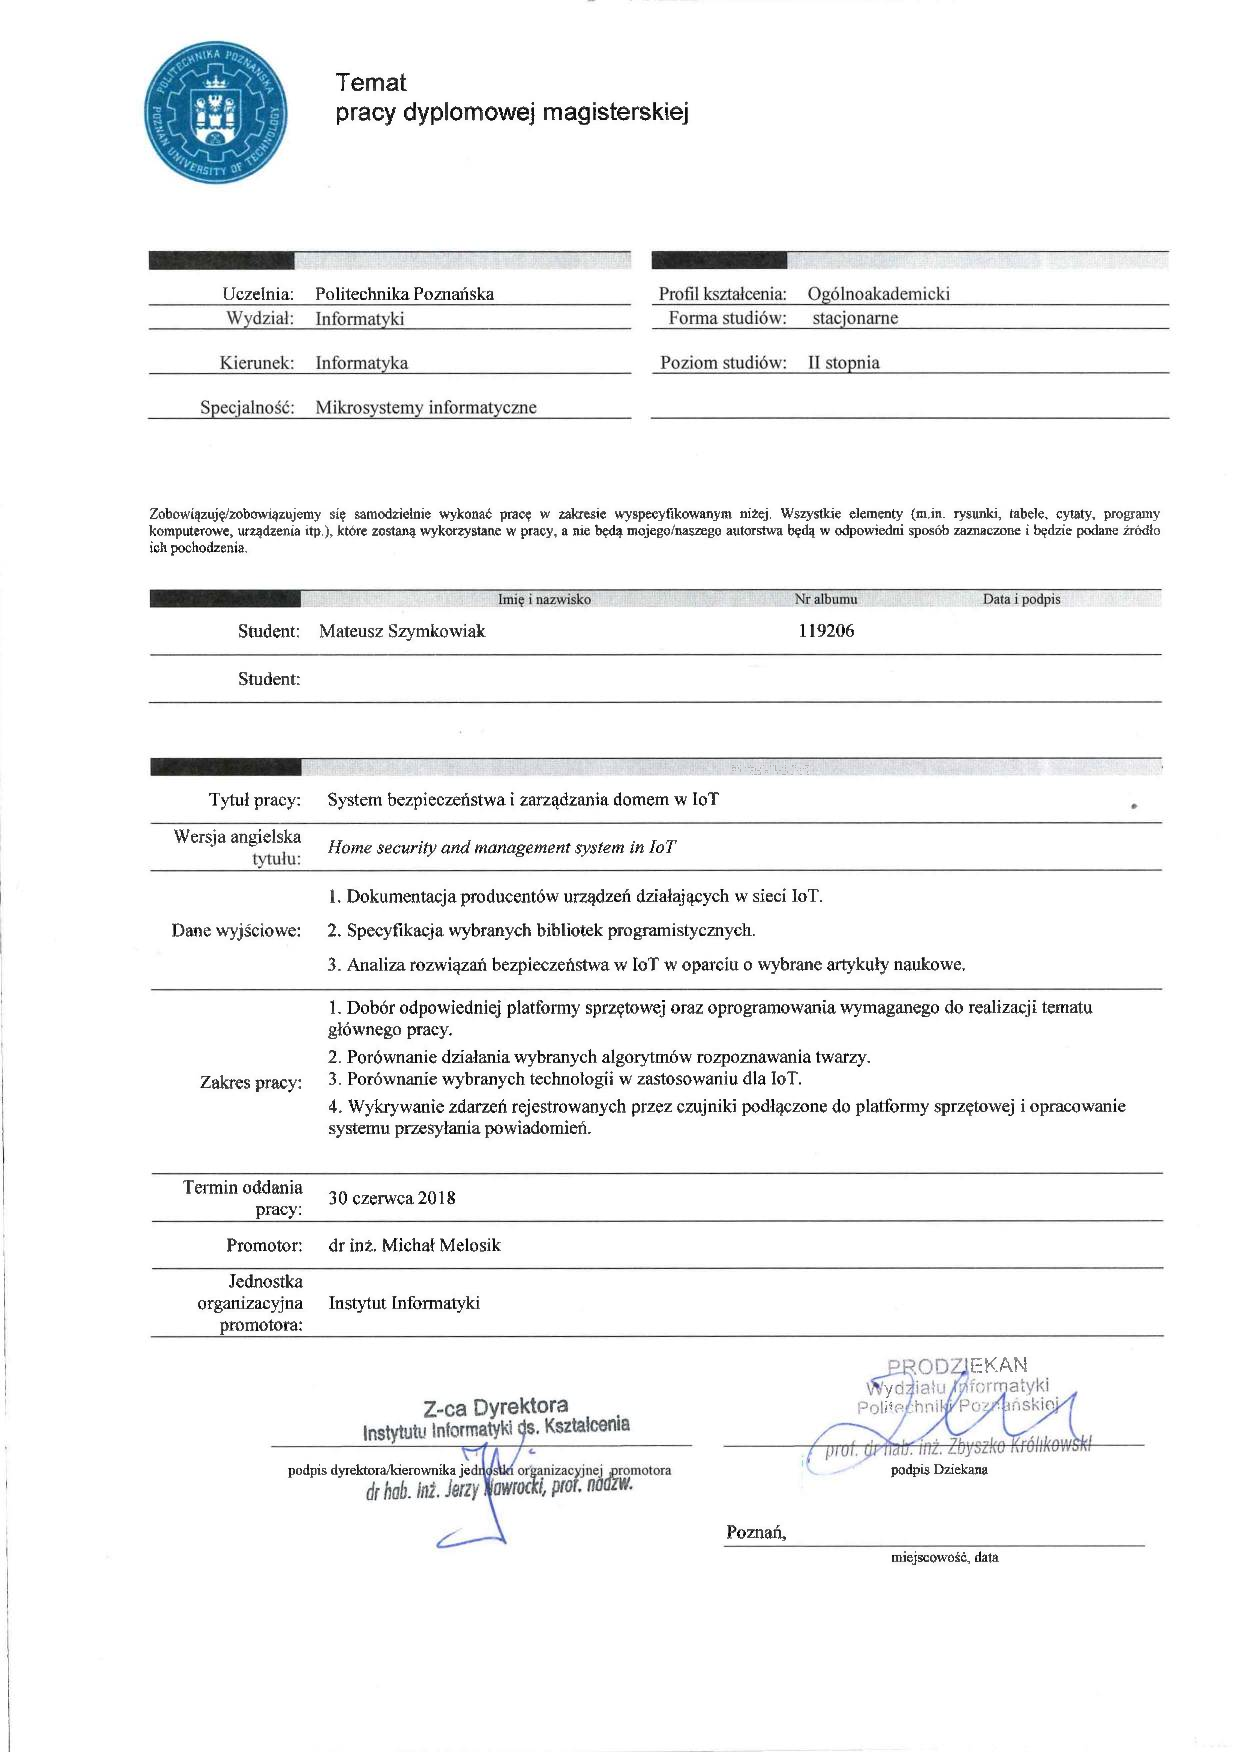
\includepdf[pages={1}]{./pictures/karta_pracy.pdf}

%%%%%%%%%%%%%%%%%%%%%%%%		STRESZCZENIE
\vspace*{\fill}
\begin{center}
{\centering \Huge \bfseries Streszczenie}\\
\end{center}
W pracy zaprezentowano system bezpieczeństwa i zarządzania domem w Internet of Things. Głównymi obiektami badań, na którym skupiono się w tej pracy są systemy detekcji oraz rozpoznawania twarzy. Na potrzeby tej pracy utworzono aplikację internetową umożliwiającą sprawne testowanie wybranych algorytmów, sieci neuronowych oraz usług pozwalających na analizę obrazu. Z powodu niewystarczającej mocy obliczeniowej platformy Raspberry Pi, przetestowano środowiska Azure oraz AWS pozwalające na uruchomienie aplikacji w chmurze.
\\
\\
\\
\begin{center}
 {\Huge \bfseries  Abstract}\\
\end{center}
english
\\
\\
\\
\\
\\
\\
\\
\\
\\
\vspace*{\fill}
%%%%%%%%%%%%%%%%%%%%%%%%		SPIS TREŚCI

\tableofcontents

%%%%%%%%%%%%%%%%%%%%%%%%	WSTĘP
\chapter{Wstęp}
Internet rzeczy (Internet of Things -IoT) to koncepcja przedstawiająca sieć urządzeń fizycznych połączonych inteligentną siecią KNX lub internetową, komunikujących się między sobą i wymieniających dane. Podstawowym celem IoT jest stworzenie inteligentnych przestrzeni- miast, budynków lub systemów związanych z życiem codziennym. Jednym z zastosowań takich systemów są inteligentne domy (smart homes), wykorzystujące czujniki oraz aktuatory do zarządzania domem.

Na potrzeby tej pracy opracowano system bezpieczeństwa oparty o system detekcji i rozpoznawania twarzy na obrazie.

%TODO dodać coś o przetwarzani obrazu, rozpoznawaniu twarzy itd

W rozdziale ,,Cel i zakres pracy'' przedstawiono główne założenia projektu oraz zakres prac autora.

W rozdziale ,,Wstęp teoretyczny'' omówiono podstawowe zagadnienia związane z treścią tej pracy magisterskiej.

W rozdziale ,,Przegląd dostępnych metod rozpoznawania twarzy'' porównano możliwości kilku z dostępnych usług lub oprogramowania pozwalającego na rozpoznawanie twarzy.

W rozdziale ,,System zarządzania metodami rozpoznawania twarzy'' przedstawiono strukturę stworzonej aplikacji, jej podział na moduły oraz wybrane dla każdego z nich środowisko uruchomieniowe.

W rozdziale ,,Aplikacja internetowa'' zaprezentowano wszystkie strony utworzone na potrzeby projektu.

W rozdziale ,,Aplikacja konsolowa'' omówiono sposób wykorzystania wcześniej opisanych usług oraz algorytmy odpowiedzialne za działanie systemu do testowania różnych rozwiązań dla problemu identyfikacji twarzy.

W rozdziale ,,Aplikacja konsolowa do zarządzania domem'' opisano sposób wykorzystania czujników oraz kamery podłączonej bezpośrednio do platformy Raspberry Pi.

W rozdziale ,,Porównanie wykorzystanych technologi'' zbadano oraz porównano skuteczność działania technologi wybranych na potrzeby tej pracy.

W rozdziale ,,Podsumowanie'' zawarto podsumowanie zgromadzonych informacji oraz przedstawiono wnioski wynikające z przeprowadzonych badań.



%TODO dodać opisy kolejnych rozdziałów


%%%%%%%%%%%%%%%%%%%%%%%%	CEL I ZAKRES PRAC
\chapter{Cel i zakres prac}
Celem pracy było stworzenie systemu bezpieczeństwa i zarządzania domem w IoT. Głównymi założeniami było opracowanie systemu pozwalającego na porównanie wybranych metod i usług pozwalających na analizę obrazu oraz kontrolę stanu czujników podłączonych do systemu. IoT jest bardzo prężnie rozwijającą się ideą, dlatego postanowiono porównać wybrane technologie i usługi ułatwiające zarządzanie oraz integrację z takimi aplikacjami.

Jako platformę sprzętową wybrano bardzo popularne w zastosowaniach IoT urządzenie Raspberry Pi 3. Z powodu jego ograniczonych zasobów obliczeniowych zintegrowano chmurowe usługi Azure oraz AWS. Zakres pracy obejmuje następujące zagadnienia:
\begin{itemize}
\item dobór odpowiedniej platformy sprzętowej oraz oprogramowania,
\item porównanie działania wybranych algorytmów detekcji oraz rozpoznawania twarzy,
\item wybór i porównanie wybranych technologi umożliwiających integrację z systemami IoT,
\item wykrywanie zdarzeń rejestrowanych przez wybrane czujniki
%TODO is it really needed?
\item opracowanie systemu przesyłania powiadomień
\item porównanie przydatności zintegrowanych usług w zastosowaniu dla systemu bezpieczeństwa domu
\end{itemize}

%%%%%%%%%%%%%%%%%%%%%%%%	Wstęp teoretyczny
\chapter{Wstęp teoretyczny}
\section{Technologie}
\subsection{Wzorzec projektowy MVC (Model-View-Controller)}
Strona internetowa powstała na bazie bardzo popularnego wśród programistów wzorca projektowego MVC. Założenia wzorca Model-Widok-Kontroler przedstawionego na rysunku \ref{fig:schemat_mvc} są bardzo proste, ich składowymi są:
\begin{itemize}
\item Model- reprezentuje logikę biznesową. Tutaj znajdują się wszelkie obiekty, które służą do wykonywania zaimplementowanej funkcjonalności danej aplikacji,
\item Widok- jest warstwą prezentacji. Odpowiada za prezentację logiki biznesowej (Modelu) użytkownikowi w przystępny sposób,
\item Kontroler- obsługuje żądania użytkownika. Odebrane zadania oddelegowuje do odpowiednich modeli.
\end{itemize}
\begin{figure}[H]
	\centering
	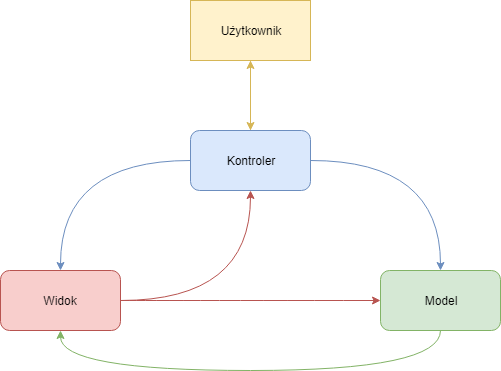
\includegraphics[scale=0.6]{mvc.png}
	\caption{Schemat klasycznego wzorca MVC}
	\label{fig:schemat_mvc}
\end{figure}

\subsection{Single Page Application}
Single Page Application (SPA) to aplikacja lub strona internetowa, która w całości wczytuje się za jednym razem. Cały potrzebny do działania strony kod (HTML, CSS, JavaScript) przesyłany jest na początku lub dodawany dynamicznie w kawałkach, zwykle w odpowiedzi na interakcje generowane przez użytkownika.
Sposób działania takiej aplikacji jest zbliżony do odczuć towarzyszących korzystaniu z aplikacji desktopowej lub mobilnej.

\subsection{Chmura obliczeniowa}
Chmura obliczeniowa jest określeniem oznaczającym model przetwarzania danych oparty na użytkowaniu usług dostarczonych przez usługodawcę. Reprezentację budowy takiego systemu przedstawiono na rysunku \ref{fig:chmura_obliczeniowa}. Użytkownik nie musi opłacać licencji, a płaci jedynie za użytkowanie danej usługi. W przypadku takich usług najpopularniejszym sposobem naliczania kosztów jest opłata od czasu użytkowania usługi.
Do najpopularniejszych udostepnianych usług należą:
\begin{itemize}
\item bazy danych,
\item maszyny wirtualne,
\item serwery,
\item hosting dla aplikacji webowych.
\end{itemize}
Przedstawicielami usługodawców udostępniających szeroki zakres usług, które zostały wykorzystane podczas tworzenia tej pracy magisterskiej jest Azure od Microsoft oraz AWS stworzony przez Amazon. Usługi obu podmiotów, które mogą być przydatne podczas tworzenia rozwiązania zostały szerzej opisane w podpunkcie \ref{azure} i \ref{aws}.
\begin{figure}[H]
	\centering
	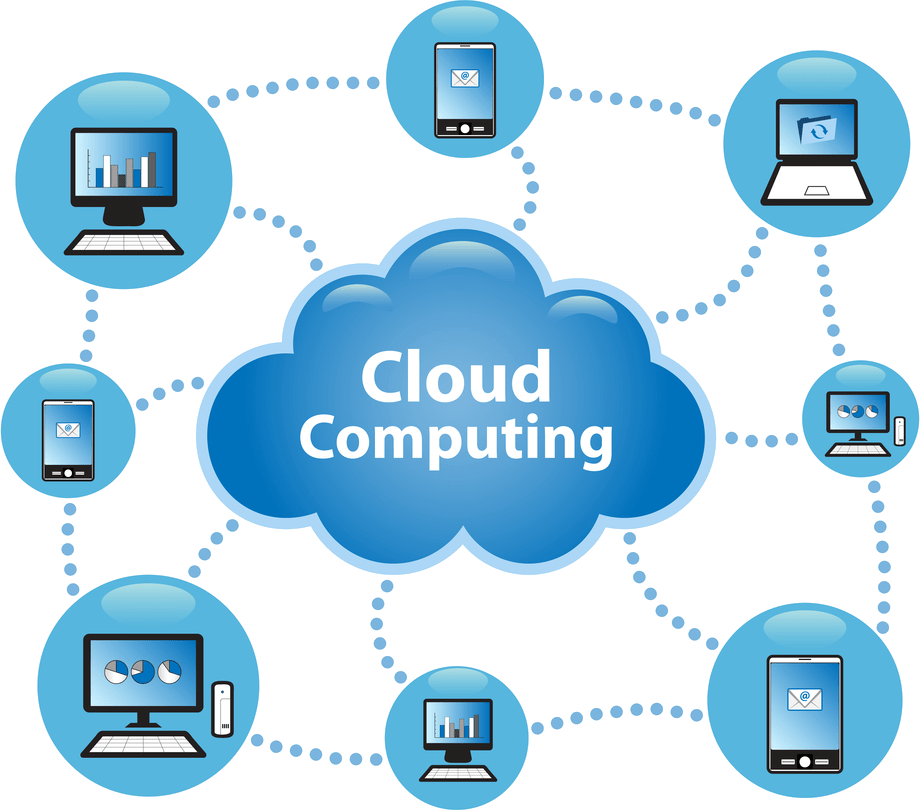
\includegraphics[scale=0.8]{cloud_computing.png}
	\captionsource{Obliczenia chmurowe}{http://www.justscience.in}
	\label{fig:chmura_obliczeniowa}
\end{figure}
\subsection{1-Wire} \label{1wire}
One Wire to systemowa magistrala komunikacji elektronicznej pomiędzy urządzeniami, zapewniająca przesyłanie danych oraz zasilanie urządzenia przez pojedynczy kabel. Proces ten jest możliwy dzięki stopniowemu ładowaniu kondensatora znajdującego się w odbiorniku, a następnie wykorzystanie zgromadzonej energii do zasilenia urządzenia. Do magistrali może zostać podłączonych wiele urządzeń. Każdemu z nich przydzielany jest indywidualny adres 64-bitowy. Komunikację z urządzeniami inicjuje master, w tym przypadku Raspberry Pi.
Przedstawiony protokół jest bardzo podobny do I2C, ale ze względu na wykorzystanie jedynie jednej linii danych, charakteryzuje się niższą prędkością przesyłania. Układ zazwyczaj zasilany jest napięciem o wartości 5V i służy do komunikacji pomiędzy niewielkimi urządzeniami, takimi jak np. termometr cyfrowy i mikrokontroler.

\section{Raspberry Pi} \label{raspi}
Raspberry Pi jest platformą komputerową stworzoną przez Raspberry Pi Foundation, na którą składa się pojedynczy obwód drukowany widoczny na zdjęciu \ref{fig:raspberrypi}. Pierwsza wersja tego urządzenia została zaprezentowana w 2012 roku. Na potrzeby tej pracy wykorzystano nowszą wersję urządzanie w wersji 3 B, którą została wyposażona w 4 rdzeniowy procesor i 1 GB pamięci RAM. Raspberry pozwala na podłączenie wielu urządzeń peryferyjnych za pomocą 4 portów USB lub 40 pinów GPIO. Dodatkowe złącze pozwala na podłączenie dedykowanej kamery. Dzięki znacznej ilości portów GPIO istnieje możliwość komunikacji cyfrowej z sensorami. Budowa urządzenia nie pozwala na podłączenie czujników analogowych.
\begin{figure}[H]
	\centering
	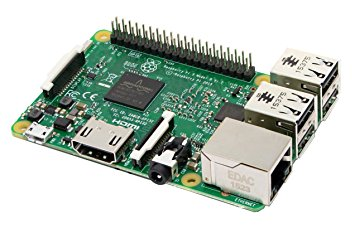
\includegraphics[scale=0.6]{raspberrypi.jpg}
	\captionsource{Raspberry Pi 3 B}{https://www.amazon.ca}
	\label{fig:raspberrypi}
\end{figure}

\subsection{Czujnik DHT 11}
\begin{figure}[H]
	\centering
	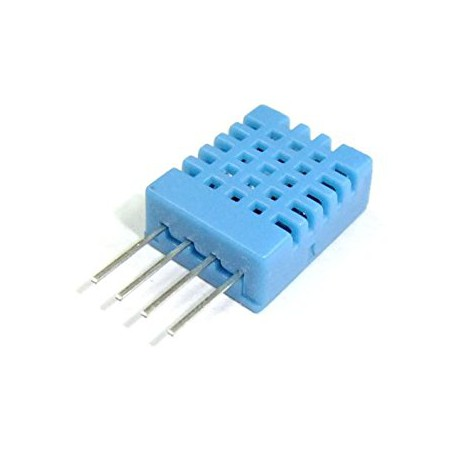
\includegraphics[scale=0.2]{dht11.jpg}
	\caption{Czujnik DHT11}
	\label{fig:dht11}
\end{figure}
Czujnik temperatury i wilgotności powietrza DHT11 jest bardzo popularnym czujnikiem z interfejsem cyfrowym. Do komunikacji wykorzystuje on protokół 1-wire opisany w rozdziale \ref{1wire}.
\begin{table}[H]
	\centering
	\caption{Parametry czujnika}
	\begin{tabular}{|c|c|}
  		\hline 
  		\bfseries Parametr & \bfseries Wartość \\
  		\hline
  		Napięcie zasilania & 3,3V do 5,5V\\
  		\hline
  		Średni pobór prądu & 0,2 mA\\
  		\hline 
  		Zakres pomiaru temperatury & od - 20\si{\degree}C do +50\si{\degree}C\\
  		\hline 
  		Zakres pomiaru wilgotności & od 5\% do 95\% wilgotności względnej\\
  		\hline 
  	\end{tabular}
\end{table}

\subsection{Raspberry Pi Camera HD}
Raspberry Pi Camera HD jest dedykowaną kamerą przeznaczoną tylko i wyłącznie do urządzenia Raspberry Pi w wersji 3, 2 oraz B+. Szybszy transfer danych niż przez port USB zapewnia dedykowane złącze minikomputera (w formie taśmy na zdjęciu \ref{fig:picamera}). Kamera posiada matrycę o rozdzielczości 8 Mpx, wspiera tryb HD 1090p, 720p oraz 640 x 480. Moduł umożliwia wykonywanie zdjęć w rozdzielczości nawet 3280 x 2464 px. Wymagane sterowniki są preinstalowane na kompatybilnych urządzeniach.
\begin{figure}[H]
	\centering
	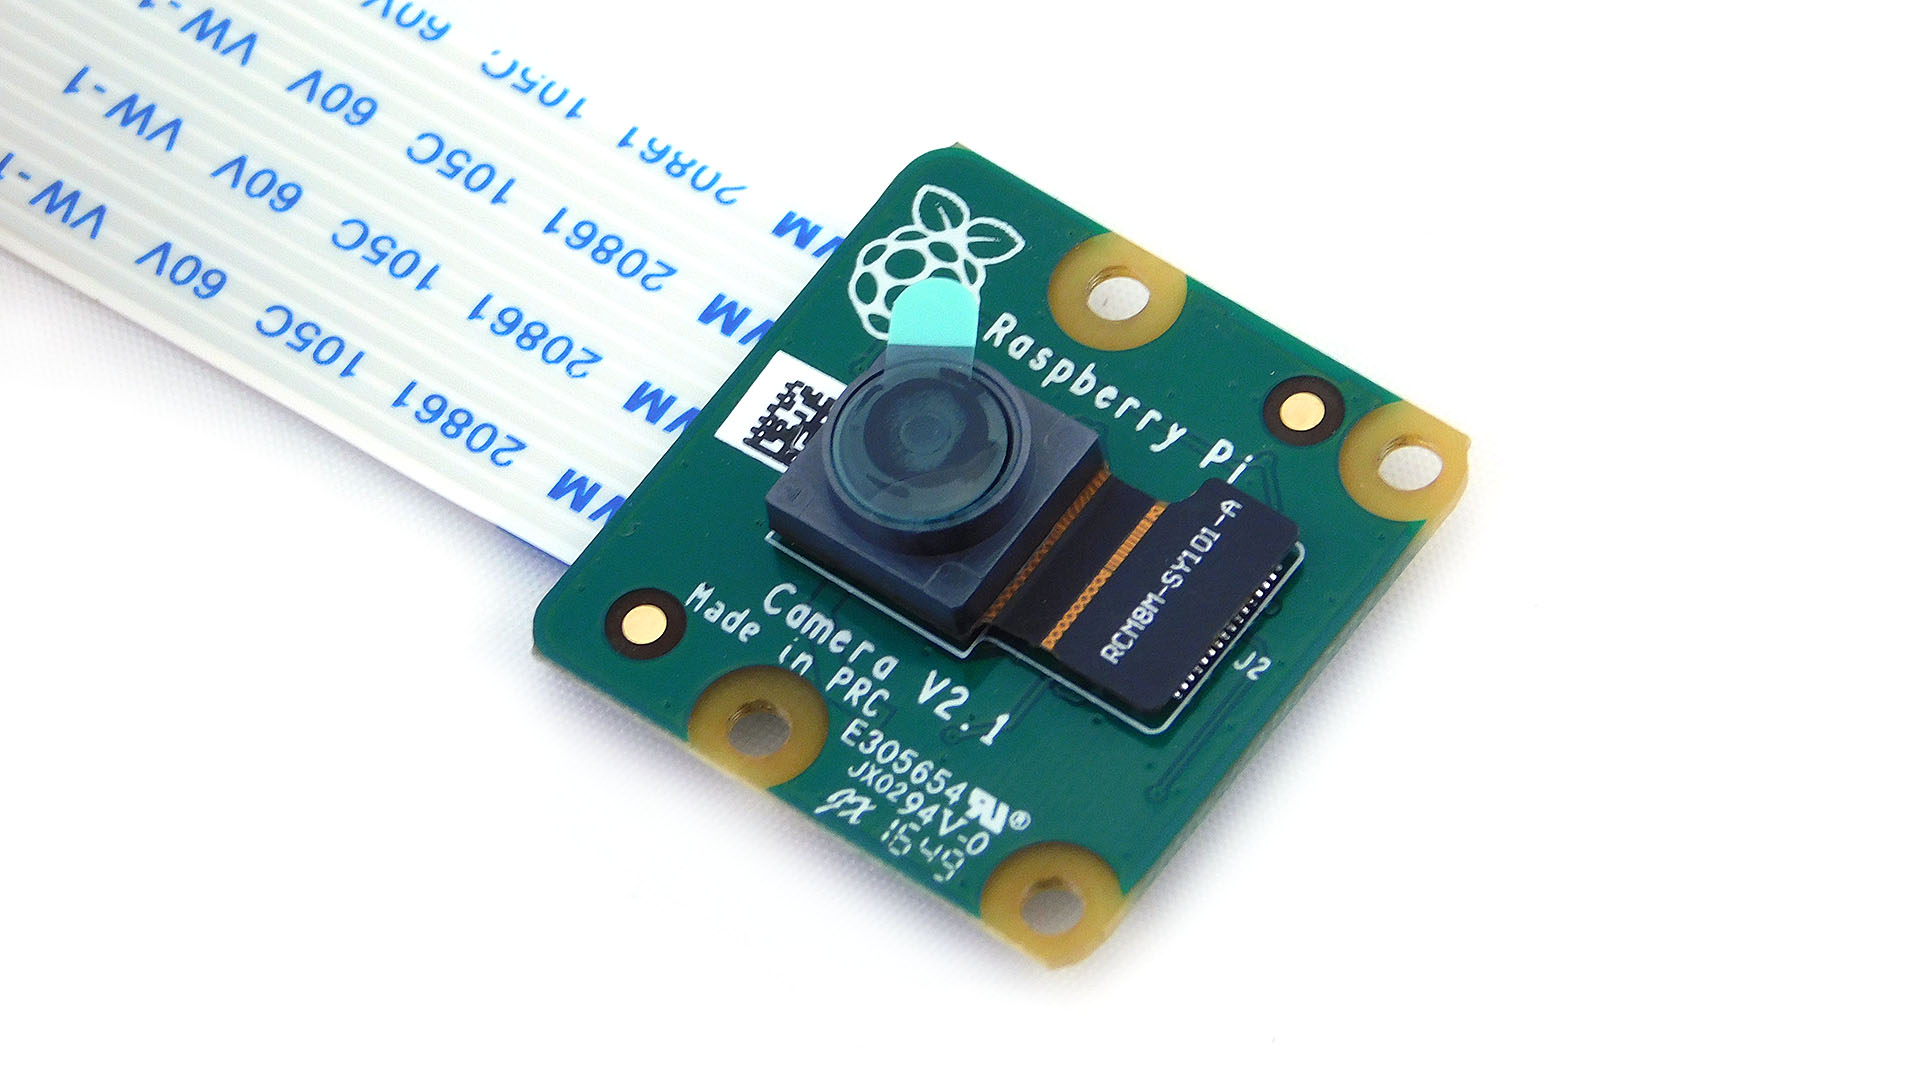
\includegraphics[scale=0.05]{picamera.jpg}
	\caption{Raspberry Pi Camera Hd}
	\label{fig:picamera}
\end{figure}

\section{Przetwarzanie obrazu}
\subsection{Thresholding \textcolor{red}{TODO}}
Thresholding jest operacją polegającą na segmentacji obrazu. Segmentacja to proces podziału obrazu na części określane jako obszary, które są jednorodne pod względem pewnych wybranych własności. Podczas thresholdingu dochodzi do porównania wartości pixeli, tak by oddzielić ważne piksele od tych mniej interesujących. Przed operacją ustalana jest granica, która będzie stanowić o tym jak rozdzielone zostaną wartości.
\begin{figure}[H]
	\centering
	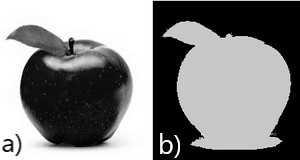
\includegraphics[scale=0.5]{efekt_thresholdingu.jpg}
	\caption{Efekt działania thresholdingu a) przed b) po}
	\label{fig:efekt_thresholdingu}
\end{figure}
Zakładając, że obraz wejściowy to $src$, wartość danego piksela oznaczono jako $src(x,y) $, a przyjętą granicę jako $thresh$. Na rysunku \ref{fig:thresholding} niebieską linią oznaczono $thresh$, a czerwonym kolorem obszar oznaczający wartość piksela. 
\begin{figure}[H]
	\centering
	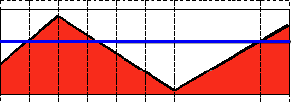
\includegraphics[scale=0.8]{thresholding.png}
	\caption{Wykres wartości obrazu $src$ przed thresholdingiem}
	\label{fig:thresholding}
\end{figure}
\begin{figure}[H]
	\centering
	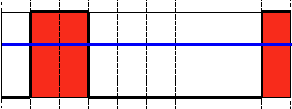
\includegraphics[scale=0.8]{thresholding_binarny.png}
	\caption{Wykres wartości pikseli obrazu $dst$}
	\label{fig:thresholding_binarny}
\end{figure}
W tej pracy zastosowano thresholding binarny konwertujący wartość każdego piksela do minimalnej lub maksymalnej. Działanie funkcji przedstawiono za pomocą poniższego wzoru.
 \begin{equation}
 \label{eq:thresholding}
 \begin{aligned}
dst(x,y) = \left\{ \begin{array}{ll}
maxValue & \textrm{gdy $src(x,y)>$thresh}\\
0 & \textrm{pozostałe}
\end{array} \right.
 \end{aligned}
\end{equation}
 \\ \textcolor{red}{POPRAWIĆ WZÓR I OPIS}gdzie maxValue- wartość maksymalna piksela
 \\ dst- plik wyjściowy \\
Porównując rysunki \ref{fig:thresholding} oraz \ref{fig:thresholding_binarny} można zaobserwować że zgodnie ze wzorem 3.1 każdy piksel obrazu wejściowego poniżej wartości $thresh$ (niebieska linia), na obrazie wyjściowym ma wartość 0, a powyżej linii ma wartość maksymalną.

\subsection{Dylatacja}
Dylatacja jest operacją wykorzystywaną do przetwarzania obrazów binarnych, określaną rozszerzaniem. Proces dylatacji polega na przyłożeniu do każdego pixela na obrazie struktury o wybranym rozmiarze. Jeżeli choć jeden piksel sąsiadujący z punktem centralnym wybranej struktury ma wartość jeden to punkt centralny również otrzymuje taką samą wartość. W przeciwnym wypadku punktowi przypisywana jest wartość zero. Najkorzystniejsze efekty przynosi dylatacja strukturą przypominającą kształt koła, np 3x3 px. W efekcie dylatacji dochodzi do zwiększenia się obiektu, zniknięcia detali oraz wypełnienia pustek w niespójnym obszarze. Na rysunku \ref{fig:dylatacja} b) do obrazu przyłożono strukturę 3x3 px. W jej obszarze znaleziono jeden piksel o wartości maksymalnej(oznaczony szarym kolorem), dlatego pikselowi oznaczonemu kolorem zielonym zostaje przydzielona ta sama wartość. Przeprowadzenie operacji na całym obrazie, powoduje uzyskanie rysunku \ref{fig:dylatacja} c).
\begin{figure}[H]
	\centering
	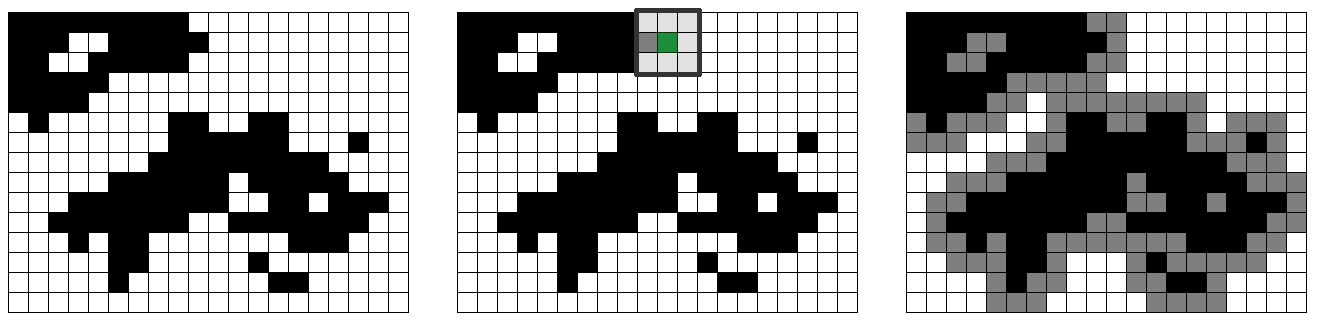
\includegraphics[scale=0.4]{dylatacja.png}
	\captionsource{Przebieg przykładowej dylatacji a) przed b) w trakcie c) po}{https://pl.wikipedia.org/wiki/Cyfrowe\_ przetwarzanie\_ obrazów\_ binarnych}
	\label{fig:dylatacja}
\end{figure}

\subsection{Rozmycie gaussowskie \textcolor{red}{DODAĆ wzór i więcej opisu}}
Rozmycie gaussowskie inaczej nazywane wygładzaniem gaussowskim to operacja przetwarzania obrazu polegająca na modyfikacji go z użyciem filtru Gaussa. Rozmycie wykorzystywane jest w celu zmniejszenia szumów oraz zakłóceń w obrazie oraz w celu zamazania detali.
\begin{figure}[H]
	\centering
	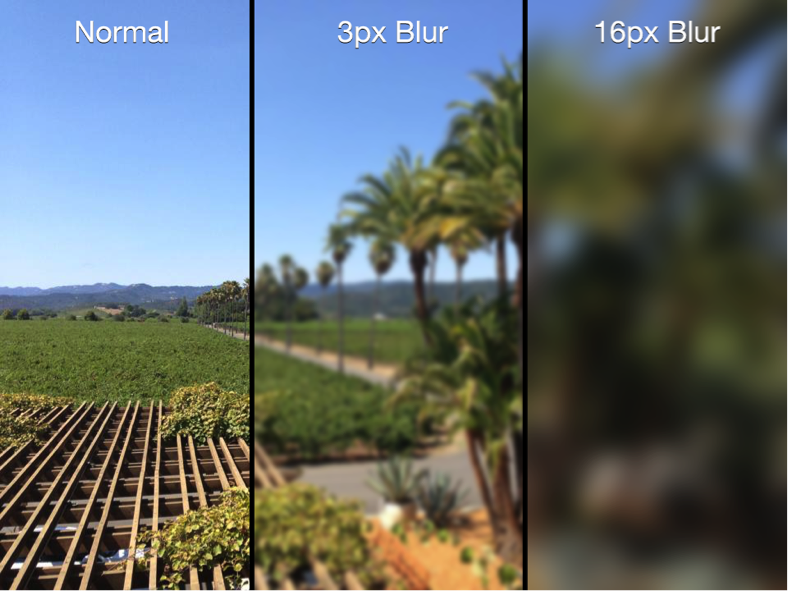
\includegraphics[scale=0.4]{rozmycie_gaussowskie.png}
	\caption{Przykład zastosowania rozmycia gaussowskiego na zdjęciu}
	\label{fig:rozmycie_gaussowskie}
\end{figure}

\subsection{Klasyfikator kaskad Haar'a} \label{haar}
Detekcja obiektów klasyfikatorem kaskad Haar'a została oparta o metodę Paul'a Viola i Michael'a Jones'a– w skrócie Viola-Jones.

Algorytm Viola-Jones jest jednym z pierwszych algorytmów pozwalających na osiągnięcie zadowalających wyników w detekcji obiektów na obrazie. Został on zaproponowany w 2001 roku i został przemyślany z głównym przeznaczeniem dla detekcji twarzy. Na kluczowe koncepcje tej metody składają się:
\begin{itemize}
\item wyszukiwanie cech Haar'a,
\item integralność obrazu,
\item metoda uczenia AdaBoost (podstawowy algorytm do boostingu, metoda dzięki której z dużej liczby słabych klasyfikatorów można otrzymać jeden lepszy )
\end{itemize}

Cechy wykorzystywane w metodzie Viola-Jones opierają się na falkach Haara. Falki Haara są to sekwencje przeskalowanych kwadrato-podobnych funkcji, które razem tworzą falę(falo-podobną oscylację), podstawę z której można zbudować kwadrat. W dwóch wymiarach, fala kwadratu jest parą przylegających do siebie prostokątów, gdzie jeden jest jaśniejszy, a drugi ciemniejszy. Podstawowe szablony przedstawiono na rysunku \ref{fig:szablon_cech_haara}.
\begin{figure}[H]
	\centering
	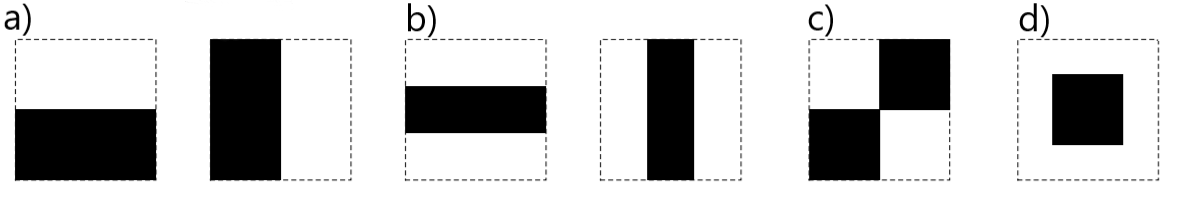
\includegraphics[scale=0.4]{szablon_cech_haara.png}
	\caption{Szablony cech Haar'a a) dwuprostokątny b) trójprostokątny c) czteroprostokątny d) centralny}
	\label{fig:szablon_cech_haara}
\end{figure}
Wartość każdej cechy jest obliczana jako różnica sumy poziomów szarości pikseli pokrywanych przez biały oraz czarny prostokąt oraz sumy poziomów szarości pikseli pokrywanych przez czarny prostokąt. Składniki tej różnicy posiadają wagi odwrotnie proporcjonalne do rozmiarów, dzięki czemu różnice wielkości dwóch obszarów są kompensowane.
\textcolor{red}{MOŻE JESZCZE WZÓR?}

\subsection{Głęboka sieć neuronowa} \label{dnn}
Pojęciem uczenia maszynowego określa się dziedzinę nauk związanych ze sztuczną inteligencją, zajmującą się badaniem algorytmów i systemów, które usprawniają swoje działanie wraz ze zdobywaniem nowej wiedzy lub też doświadczeniem. Wiedzą określamy dane uczące, które zostały wykorzystane do nauki. System może zostać usprawniony poprzez zwiększenie wiedzy systemu, które powinno pozwolić na usprawnienie procesu rozwiązywania podstawowych problemów.
\begin{figure}[H]
	\centering
	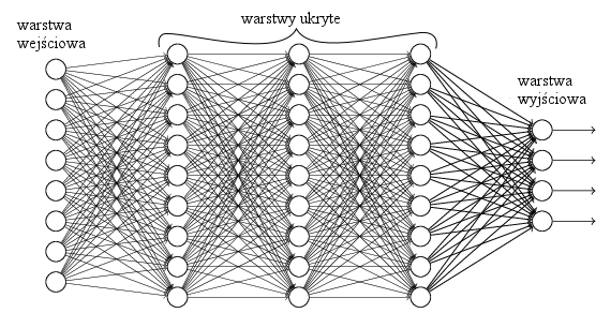
\includegraphics[scale=0.6]{schemat_dnn.png}
	\caption{Budowa głębokiej sieci neuronowej}
	\label{fig:budowa_dnn}
\end{figure}
Algorytmy głębokiego uczenia maszynowego są jednymi z najbardziej zaawansowanych. Zbudowane są one w sposób przypominający biologiczne sieci neuronowe. Głęboka sieć neuronowa składa się z neuronów rozmieszczonych na warstwach. Wiele warstw jest powodem dla którego taki rodzaj algorytmu określa się mianem głębokiego. Przykładowa budowa głębokiej sieci neuronowej została przedstawiona na rysunku \ref{fig:budowa_dnn}.

Każdy z takich “sztucznych neuronów” jest tak naprawdę informacją, która jest przesyłana dalej do następnych neuronów i ich warstw. Poszczególne warstwy “uczą” się przetwarzać kolejne cechy obiektów/obrazów/dźwięków itp., dzięki czemu są w stanie odtwarzać całe obiekty w bardzo rzeczywisty sposób. W tej pracy wykorzystano głęboką sieć neuronową do zadania wykrywania twarzy na obrazie.

\section{Azure} \label{azure}
Azure jest platformą chmurową firmy Microsoft stworzoną w modelu Paas (Platform as a Service). Platforma zbudowana jest z grupy trzech technologii zapewniających specjalizowany zestaw możliwości dla programistów, które mogą być wykorzystywane zarówno przez aplikacje uruchamiane lokalnie na komputerach użytkowników oraz aplikacje uruchamiane w chmurze. W tej pracy wykorzystano:
\begin{itemize}
    \item App Services,
    \item Azure Cognitive Services,
    \item bazy danych SQL oraz NoSQL (MSSQL, MySql, CosmicDB)
    \item maszyny wirtualne oparte o system Windows oraz kilka popularnych dystrybucji Linuxa.
\end{itemize}
\subsection{Web App Services}
Web App Services jest usługą pozwalającą na hostowanie aplikacji internetowych napisanych w jednym z wybranych języków (między innymi .Net, Node.Js, Python) bez zarządzania infrastrukturą. Do największych zalet należy automatyczna skalowalność serwisu oraz wysoka dostępność. Podczas tworzenia środowiska istnieje możliwość wyboru preferowanego systemu operacyjnego. Dużą zaletą jest możliwość wdrożenia aplikacji za pomocą jednego kliknięcia bezpośrednio z Visual Studio. Sprawne korzystanie z usługi jest możliwe dzięki szerokiemu zakresowi dokumentacji i tutoriali udostepnionych przez producenta.

\section{AWS} \label{aws}
Amazon Web Services jest platformą chmurową firmy Amazon stworzoną w modelu Paas (Platform as a Service). Jest to bardzo podobne rozwiązanie do bliźniaczego Azure. Platforma udostępnia obliczenia chmurowe na żądanie. Szeroki zakres usług dostępny jest w darmowej wersji demo, jedynym wymaganiem jest założenie konta w serwisie. Po wykorzystaniu darmowego okresu, opłaty naliczane są według zużycia danej usługi. Do podstawowych usług, które mogłyby zostać wykorzystane dla celów tej pracy należą:
\begin{itemize}
    \item Elastic Beanstalk,
    \item Rekognition,
    \item bazy danych (RDS),
    \item maszyny wirtualne (EC2).
\end{itemize}
\subsection{Elastic Beanstalk}
Elastic Beanstalk jest odpowiednikiem Azure Web App Services. Zakres dostępnych języków jest równie szeroki jak w przypadku Azure'a, ale w odróżnieniu od Microsoftu nie zawsze wspiera on najnowszych wersji produktów wymienionej firmy, a zakres możliwości konfiguracyjnych z poziomu strony internetowej jest uboższy. Podobnie jak w przypadku Azure istnieje możliwość wdrożenia aplikacji jednym kliknięciem po doinstalowaniu dedykowanego pluginu do Visual Studio.

%%%%%%%%%%%%%%%%%%%%%%%%	Przegląd dostępnych metod rozpoznawania twarzy
\chapter{Przegląd dostępnych metod rozpoznawania twarzy}
Przez ostatnie lata dziedzina cyfrowego przetwarzania obrazu bardzo prężnie rozwijała się. W wyniku tego aktualnie dostępnych jest wiele usług pozwalających na uzyskiwanie danych z obrazu. W przypadku tej pracy najbardziej użytecznymi informacjami jest lokalizacja oraz identyfikacja twarzy.
Na rysunku \ref{tab:systemy} przedstawiono cechy kilku wybranych systemów, stworzonych przez jedne z największych firm zajmujących się technologiami informatycznymi na świecie.

\begin{table}[H]\label{tab:systemy}
	\centering
	\caption{Dostępne systemy przetwarzania obrazu}
	\scalebox{0.75}{
	\begin{tabular}{|c|c|c|c|c|c|c|}
  		\hline 
  		 & \bfseries OpenCv & \bfseries Azure CS & \bfseries AWS Rekognition & \bfseries Google & \bfseries face recognition & \bfseries open face\\
  		\hline
  		\bfseries Detekcja twarzy &tak&tak&tak&tak&tak&tak\\
  		\hline
  		\bfseries Identyfikacja twarzy &tak&tak&tak&nie&tak&tak\\
  		\hline
  		\bfseries Rozpoznawanie emocji &nie&tak&nie&nie&nie&nie\\
  		\hline
  		\bfseries SDK &tak&tak&tak&tak&Python&Python\\
  		\hline
  		\bfseries API &nie&tak&tak&tak&nie&nie\\
  		\hline
  		\bfseries licencja &open source&płatna/demo&płatna/demo&płatna/demo&open source&open source\\
  		\hline
  	\end{tabular}
  	}
\end{table}
Zgodnie ze wzrostem popularności usług chmurowych, aktualnie dostępnych jest wiele usług rozpoznawania twarzy, które początkowo były dostępne za pomocą API(Application Programming Interface). Z czasem większość z nich udostępniła również SDK(Software Development Kit) dla najbardziej popularnych języków (między innymi C\#, Java, Python). OpenCv \cite{opencv_doc} jest podstawową open sourcową bibliotekę pozwalającą na identyfikację twarzy. Większość darmowych rozwiązań dostępnych jest na platformie GitHub:
\begin{itemize}
\item face\_ recognition \cite{face_reco_github},
\item open face \cite{open_face}.
\end{itemize}
Niestety żadna z nich nie mogła równać się dojrzałością podobną do OpenCv, a na dodatek większość z nich
można wykorzystać jedynie tworząc oprogramowanie w języku Python.

Poza usługami przedstawionymi w tabeli \ref{tab:systemy}, równie ciekawym rozwiązaniem, aczkolwiek znacznie bardziej rozbudowanym i czasochłonnym jest wykorzystanie Tensorflow \cite{tensorflow} (framework do machine learningu) w celu zbudowanie własnej implementacji sieci neuronowej rozpoznającej twarze.
Podstawowym frameworkiem, o którego użyciu zadecydowano zostało OpenCv. Za wyborem tej biblioteki przemawiała licencja open source, dojrzałość frameworku oraz liczne źródła wiedzy o implementacji. Podstawowe dostępne funkcje i zastosowania opisano w rozdziale \ref{s:open_cv}.

W celu możliwości porównania rozwiązań lokalnych i chmurowych za drugi obiekt badań obrano usługę Azure Cognitive Services \cite{azure}, którą szerzej opisano w rozdziale \ref{azurecs}. O wyborze tego rozwiązania zadecydowała rozbudowana dokumentacja usługi oraz licencja studencka umożliwiająca darmowe wykorzystanie usługi przy zwiększonych limitach zapytań.

\section{Open Cv} \label{s:open_cv}
OpenCv (Open Source Computer Vision Library) jest open sourcową biblioteką napisaną w języku C. Udostępniono liczne interfejsy biblioteki pozwalające na pracę z nią miedzy innymi w języku C++ i Python. Biblioteka wspiera systemy operacyjne Linux oraz Windows. Biblioteka została ukierunkowana na przetwarzanie obrazu w czasie rzeczywistym. W licznie udostępnionych funkcjach można znaleźć moduły pozwalające na detekcję i rozpoznawanie twarzy na obrazie, które zostały szerzej opisane w kolejnym punkcie.

\subsection{Rozpoznawanie twarzy \textcolor{red}{ZRODŁA WZORY I CYTOWANIA}}
Przed zidentyfikowaniem tożsamości, należy najpierw rozwiązać problem detekcji twarzy. Podstawowym sposobem detekcji twarzy wykorzystywanym przez OpenCv jest kaskadowy klasyfikator Haar'a oparty o cechy Haar'a opisane w rozdziale \ref{haar}. Do innych dostępnych rozwiązań wykorzystanych do stworzenia aplikacji należy wytrenowany model głębokiej sieci neuronowej przygotowany przez autorów biblioteki.
\subsubsection{Eigenfaces} \label{eigen}
Eigenfaces, inaczej nazywany algorytmem twarzy własnych opiera się na metodzie analizy głównych składowych, która rozpoczyna się wyznaczeniem średniej wartości dla obrazów z tą samą etykietą identyfikującą daną osobę.
Weźmy $n$ wektorów $x_{i}$ powstałych jako reprezentacje obrazów przedstawiających daną twarz. Dla tych wektorów wyznaczona zostaje wartość średnia $\mu$.
$$
\mu=\frac{1}{n}\sum_{i=1}^{n}x_{i}
$$
Następnie dla każdego wektora $x_{i}$ wyznaczana jest różnica od wartości średniej $\mu$.
$$
\psi= x_{i}-\mu
$$
Na podstawie wartości $\psi_{i}$ wyznacza się macierz kowariancji $C$.
$$
C=\frac{1}{n}\sum_{i=1}^{n}\psi_{i}\psi_{i}^{T}
$$
Kolejnym krokiem jest wyznaczenie wartości $\lambda_{i}$ oraz $\nu_{i}$ tak by spełniony był warunek:
$$
C\nu_{i}=\lambda_{i}\nu_{i} \textrm{ dla $i=$1,2,...,n}
$$
Wartość $\lambda_{i}$ nazywana wartością własną amcierzy $C$, a odpowiadający jej wektor $\nu_{i}$ wektorem własnym $C$.
W przypadku algorytmu Eigenfaces branych jest pod uwagę $k$ głównych składowych $\lambda_{i}$, wyznaczonych na podstawie odrzucenia $n-k$ wartości najmniejszych. Dla każdego wektora wyznaczany jest wektor następujący:
$$
y_{i}=W^{T}(x_{i}-\mu) \textrm{ gdzie $W=(\nu_{1}, \nu_{2}, ..., \nu_{k})$}
$$
Identyfikacja twarzy algorytmem Eigenfaces polega na wykonaniu kroków:
\begin{enumerate}
\item Wartości głównych składowych zostają wyznaczone dla wszystkich obrazów uczących.
\item Wartość głównych składowych zostaje wyznaczona dla badanego zdjęcia
\item Dla obrazu wejściowego zostaje wyznaczony wektor najbliższy dla wartości obliczonych dla obrazów z bazy danych.
\end{enumerate}

\subsubsection{Fisherfaces} \label{fisher}
Algorytm Fisherfaces opiera się na liniowej analizie dyskryminacyjnej (LDA) i polega na wyznaczeniu wektora cech pozwalającego na rozdzielenie obiektów przynależnych do różnych klas. W przypadku problemu rozpoznawania twarzy, przez klasy obiektów rozumiane są zbiory obrazów przedstawiające tego samego użytkownika. Problem sprowadza się do wyznaczenia wektora, który stanowi przybliżoną granicę między dwiema klasami obiektów, jednak można go uogólnić do problemu wieloklasowego.
Wyznaczanie poszukiwanego wektora rozpoczyna się od wyznaczenia wartości średniej $\nu$ wszystkich obiektów znajdujących się w rozpatrywanym zbiorze, oraz wartości średniej $\nu_{i}$ wewnątrz poszczególnych klas. 
$$
\mu=\frac{1}{N}\sum_{i=1}^{N}x_{i}
$$
Gdzie $N$ oznacza liczebność rozpatrywanego zbioru $x_{i}$
$$
\mu_{i}=\frac{1}{|X_{i}|}\sum_{x_{j}eX_{i}}x_{j}
$$
Gdzie $X_{i}$ jest klasą obiektów o indeksie $i$, dla $i=1,2,...,n$ dla $n$ oznaczającego liczbę klas. Następnie wyznaczana jest macierz rozproszenia wewnątrzklasowego $S_{B}$ oraz macierz średniego rozproszenia wewnątrzklasowego $S_{W}$.
$$
S_{B}=\sum_{i=1}^{n}N_{i}(\mu-\mu_{i})(\mu-\mu_{i})^{T}
$$
$$
S_{W}=\sum_{i=1}^{n}\sum_{x_{j}eX_{i}}(x_{j}-\mu_{i})(x_{j}-\mu_{i})^{T}
$$
Rozwiązanie problemu sprowadza się do znalezienia danych, które pozwolą na otrzymanie największej wartości określającej stosunek rozproszenia wewnątrzklasowego do średniego wewnętrznego rozproszenia klas. Stąd algorytm poszukuje wektora $d$, dla którego poniższa funkcja osiąga maksimum.
$$
f(d)=\frac{d^{T}S_{B}d}{d^{T}S_{W}d}
$$
W celu zmniejszenia złożoności problemu, stosuje się modyfikację powyższego kryterium, wykorzystując macierz $W$ złożona z $k$ głównych wektorów własnych wyznaczonych dla macierzy kowariancji $C$ wszystkich elementów zbioru.
$$
f(d)=\frac{d^{T}W^{T}S_{B}d}{d^{T}S_{W}d}
$$
Znalezienie wektora $d$ pozwala na wyznaczenie optymalnego kierunku rozdzielającego dwie klasy obiektów.

\subsubsection{Local Binary Patterns Histograms} \label{lbph}
W odróżnieniu od holistycznego podejścia w dwóch poprzednich metodach, algorytm histogramów lokalnych binarnych wzorców wykorzystuje lokalne cechy przetwarzanych obiektów.
Dla każdego piksela wyznaczany jest ciąg binarny na podstawie porównania wartości z każdym z sąsiadów. W przypadku, gdy jego wartośc jest większa wtedy przyjmuje wartość 1, a 0 w przypadku przeciwnym. Stąd dla każdego piksela wyznaczana jest wartość $p$-znakowego binarnego ciągu, nazywanego lokalnym binarnym wzorcem.  Wyznaczanie można przeprowadzić w otoczeniu o dowolnym promieniu. W ogólności wartość funkcji LBP dla piksela o współrzędnych $(x_{c},y_{c})$ wyznacza się następująco: 
$$
LBP(x_{c},y_{c})=\sum_{p=0}^{p-1}2^{p}S(i_{p}-i_{c})
$$
Gdzie $p$ jest rozmiarem rozpatrywanego sąsiedztwa o środku w punkcie $(x_{c},y_{c})$ i jasności o wartości $i_{c}$, a $i_{n}$ jest wartością jasności dla $n$- tego punktu sąsiedztwa.
$S(x)$ jest funkcją znaku definiowaną następująco:
$$
S(x) = \left\{ \begin{array}{ll}
1 & \textrm{ dla $x>0$}\\
0 & \textrm{ w p.p.}
\end{array} \right.
$$
Działanie algorytmu polega na podzieleniu obrazu wejściowego na $m$ różnych części i wyznaczenia dla niego wartości LBP jasności pikseli. Następnie dla każdego regionu wyznaczany jest histogram wyliczonych wartości. Tak wyznaczone wartości są konkatenowane do postaci wektora.
Dla próbki wejściowej zostaje wyznaczony wektor histogramów, który następnie jest porównywany z wektorami obrazów użytych do uczenia sieci. Przewidywana etykieta jest wyznaczana na podstawie etykiety wektora najbliższego sąsiada.

\section{Azure Cognitive Services}\label{azurecs}
Cognitive Services jest częścią platformy Azure stworzonej przez Microsoft. Usługa jest płatna, ale w przypadku użytku na potrzeby studenckie przyznawany jest darmowy dostęp na ograniczony czas. Cognitive Services zajmuje się rozwiązywaniem problemów biznesowych dzięki sztucznej inteligencji. Do dostępnych modułów między innymi należą:
\begin{itemize}
\item obraz- algorytmy przetwarzania obrazów umożliwiające inteligentne identyfikowanie, podpisywanie i moderowanie grafik,
\item mowa- konwertowanie wypowiedzi audio na tekst, weryfikacja głosowa,
\item język- przetwarzanie języka naturalnego.
\end{itemize}
Na cele tego projektu wykorzystano moduł dotyczący przetwarzania obrazu, a dokładniej funkcjonalność wykrywania i rozpoznawania twarzy. Producent zadbał o możliwość integracji z większością popularnych języków programistycznych poprzez udostępnienie paczek deweloperskich. W przypadku braku SDK(Software Development Kit) dla wybranego języka istnieje możliwość skorzystania z udostępnionego REST Api. Na stronie producenta można znaleźć obszerną dokumentację \cite{acs_doc} oraz tutoriale.

\subsection{Detekcja twarzy}
Detekcja twarzy opiera się o pojedyncze zapytane do Api Azure'a. Dobierając odpowiednie parametry wejściowe klient może uzyskać dodatkowe informacje związane z przesłanym zdjęciem. W podstawowym przypadku odpowiedź serwisu ogranicza się do przydzielenia identyfikatora dla twarzy oraz obszaru zawierającego twarz w postaci JSON'a.

\subsection{Rozpoznawanie twarzy}
Na potrzeby rozpoznawania twarzy stworzono funkcja LargeGroup, która odpowiada za zarządzanie grupami ludzi/profili. Użytkownik może dodać dowolną ilość osób do grupy, a następnie przypisać wybrane zdjęcia do tożsamości.Na podstawie utworzonej grupy zostaje stworzony model umożliwiający rozpoznawania tożsamości osób w niej zawartej. Sposób wykorzystania tej usługi został znacznie szerzej opisany w rozdziale \ref{trenowanie_azure}. Sposób działania usługi bazuje nauczeniu maszynowym.

\section{AWS Rekognition}
Usługa Rekognition jest odpowiednikiem Azure Cognitive Services ograniczonym do rozwiązań związanych z przetwarzaniem obrazu i video. Do wielu dostępnych funkcji należy analiza obrazu, detekcja twarzy i tekstu, porównywanie oraz rozpoznawanie twarzy. Dla wybranych języków programistycznych udostępniono SDK oraz obszerną dokumentację z licznymi przykładami kodu.


%%%%%%%%%%%%%%%%%%%%%%%%	Budowa systemu
\chapter{System zarządzania metodami rozpoznawania twarzy}
\begin{figure}[H]
	\centering
	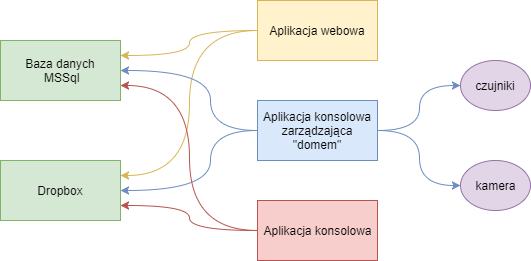
\includegraphics[scale=0.8]{schemat_systemu.png}
	\caption{Budowa systemu zarządzania domem}
	\label{fig:schemat_systemu}
\end{figure}
Aplikację powstałą na potrzeby tej pracy można podzielić na 3 moduły, które zostały przedstawione na rysunku \ref{fig:schemat_systemu}, a składają się na nie :
\begin{itemize}
\item Aplikacja webowa- interfejs pozwalający na zlecanie nowych zadań aplikacji konsolowej oraz odczyt wyników przesłanych przez nią oraz przez program zarządzający domem,
\item Aplikacja konsolowa- przetwarza zadania detekcji oraz rozpoznawania twarzy zlecone za pomocą aplikacji webowej,
\item Program zarządzający domem- przekazuje cyklicznie odczytywane dane z czujników oraz wykryte ruchy do bazy danych, w celu dalszej obróbki przez pozostałe moduły.
\end{itemize}
Na usługi pomocnicze wykorzystane w projekcie składają się
\begin{itemize}
\item baza danych- przechowywanie danych o dodanych zadaniach, wynikach, nauczonych sieciach neuronowych oraz osobach,
\item dropbox- przechowywanie większych plików- obrazów oraz nauczonych modeli sieci.
\end{itemize}

\section{Aplikacja webowa}
Aplikacja webowa jest jedyną częścią systemu, do której użytkownik może mieć bezpośredni dostęp. Strona powstała w celu maksymalnego uproszczenia procesu badania kolejnych algorytmów i usług, które różniły się sposobem podawania danych wejściowych, sposobem uczenia oraz formatem zwracanych odpowiedzi. Do pozostałych zalet takiego rozwiązania należy ułatwienie przechowywania danych, poprzez umieszczenie ich we wspólnym miejscu co pomaga, w późniejszej interpretacji wyników.
\begin{figure}[H]
	\centering
	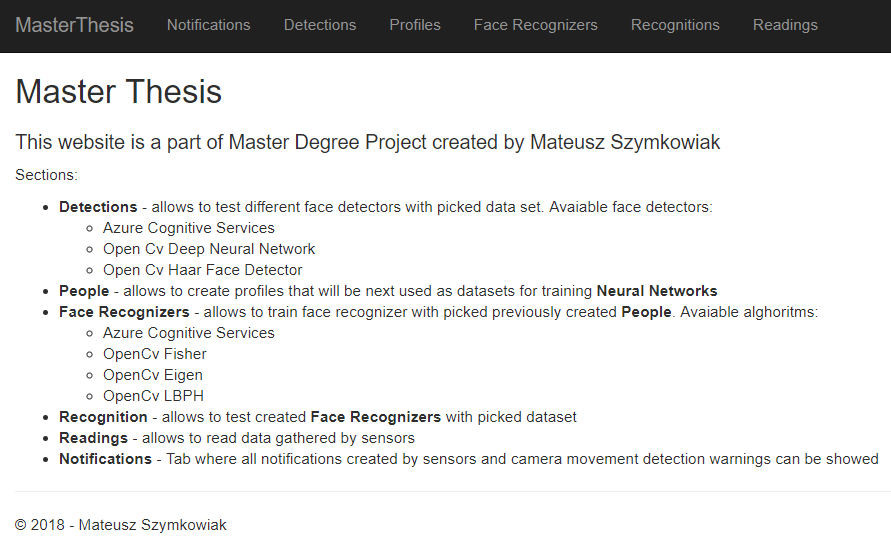
\includegraphics[scale=0.7]{aplikacja_webowa_razor_widok.png}
	\caption{Wygląd strony głównej}
	\label{fig:strona_glowna_razor}
\end{figure}
Zgodnie z interfejsem przedstawionym na rysunku \ref{fig:strona_glowna_razor}, strona została podzielona na 5 głównych sekcji:
\begin{itemize}
\item Detections- detekcje,
\item People- ludzie,
\item Neural Networks- sieci neuronowe,
\item Recognition- rozpoznawanie,
\item Sensor Readings- odczyty sensorów.
\end{itemize}

\subsection{Technologie}
Aplikacja webowa powstała w najnowszej kompilacji .NET Core 2, będącej międzyplatformową strukturą open source o wysokiej wydajności służącą do tworzenia nowoczesnych aplikacji internetowych opartych na usługach chmurowych. Logika biznesowa aplikacji została zaprogramowana w języku C\#. Warstwa widoku powstała w dwóch dostępnych rozwiązaniach, nieznacznie różniących się wyglądem, ale znacznie odbiegających od siebie sposobem działania. Przed omówieniem poszczególnych rozwiązań przedstawiono, krótkie definicje wykorzystanego wzorca projektowego MVC oraz technologii SPA

\subsubsection{Wzorzec projektowy MVC}
\begin{figure}[H]
	\centering
	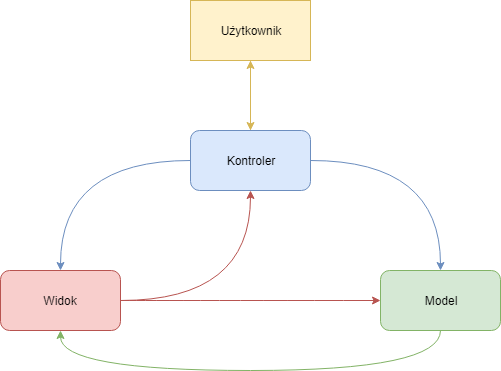
\includegraphics[scale=0.8]{mvc.png}
	\caption{Schemat klasycznego wzorca MVC}
	\label{fig:schemat_mvc}
\end{figure}
Strona internetowa powstała na bazie bardzo popularnego wśród programistów wzorca projektowego MVC. Założenia wzorca Model-Widok-Kontroler są bardzo proste, ich składowymi są:
\begin{itemize}
\item Model- reprezentuje logikę biznesową. Tutaj znajdują się wszelkie obiekty, które służą do wykonywania zaimplementowanej funkcjonalności danej aplikacji,
\item Widok- jest warstwą prezentacji. Odpowiada za prezentację logiki biznesowej (Modelu) użytkownikowi w przystępny sposób,
\item Kontroler- obsługuje żądania użytkownika. Odebrane zadania oddelegowuje do odpowiednich modeli.
\end{itemize}

\subsubsection{Single Page Application}
Single Page Application (SPA) to aplikacja lub strona internetowa, która w całości wczytuje się za jednym razem. Cały potrzebny do działania strony kod (HTML, CSS, JavaScript) przesyłany jest na początku lub dodawany dynamicznie w kawałkach, zwykle w odpowiedzi na interakcje generowane przez użytkownika.
Sposób działania takiej aplikacji jest zbliżony do odczuć towarzyszących korzystaniu z aplikacji desktopowej lub mobilnej. 

\subsubsection{Rozwiązanie 1- Razor Pages}
Pierwsza wersja została oparta o strony tworzone w technologi Razor Pages opartej o składnię Razor oraz podstawowe technologie webowe: HTML i CSS. Taki sposób tworzenia warstwy prezentacji jest zalecany dla aplikacji .NET Core, ponieważ pozwala zminimalizować ilość pracy wymaganej na jej utworzenie oraz zapewnia bardzo prosty proces wdrożenia. Aplikacja utworzona z pomocą Razor'a została zaprezentowana na rysunku \ref{fig:strona_glowna_razor}.

\subsubsection{Rozwiązanie 2- Angular 4}
Druga wersja widoku aplikacji oferuje dostęp do tych samych możliwości co pierwsze rozwiązanie, ale powstała przy pomocy frameworka webowego- Angular 4. Strona główna widoczna jest na rysunku \ref{fig:strona_glowna_angular}. Angular jest open sourcowym frameworkiem używanym do tworzenia aplikacji SPA (Single Page Application), napisany w języku TypeScript i wspierany oraz rozwijany przez Google.
\begin{figure}[H]
	\centering
	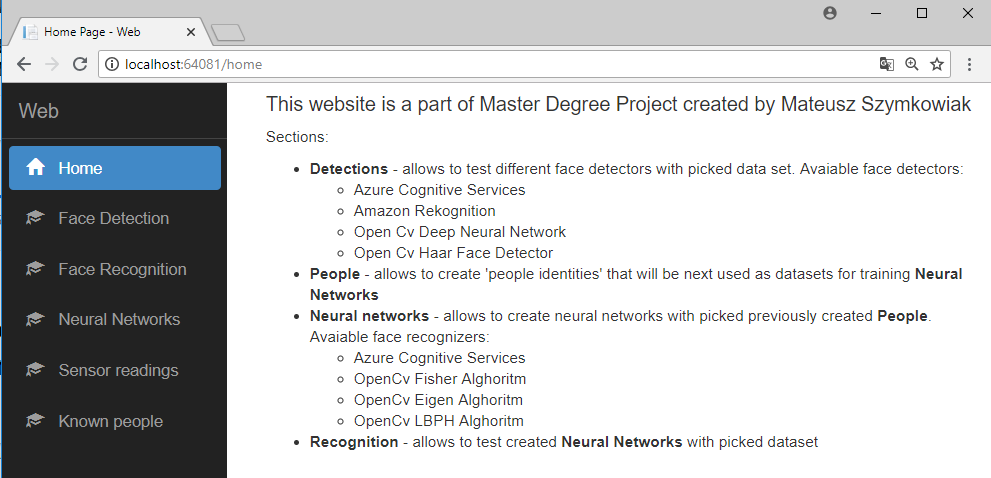
\includegraphics[scale=0.6]{aplikacja_webowa_angular_widok.png}
	\caption{Strona główna widoku utworzonym w Angular 4}
	\label{fig:strona_glowna_angular}
\end{figure}

\subsection{Detections}
Detections jest stroną odpowiedzialną za wykrywanie twarzy na obrazach przesłanych do systemu. Na głównej stronie możemy zobaczyć wszystkie zlecone detekcje, zarówno nowe jak i już zakończone.
\begin{figure}[H]
	\centering
	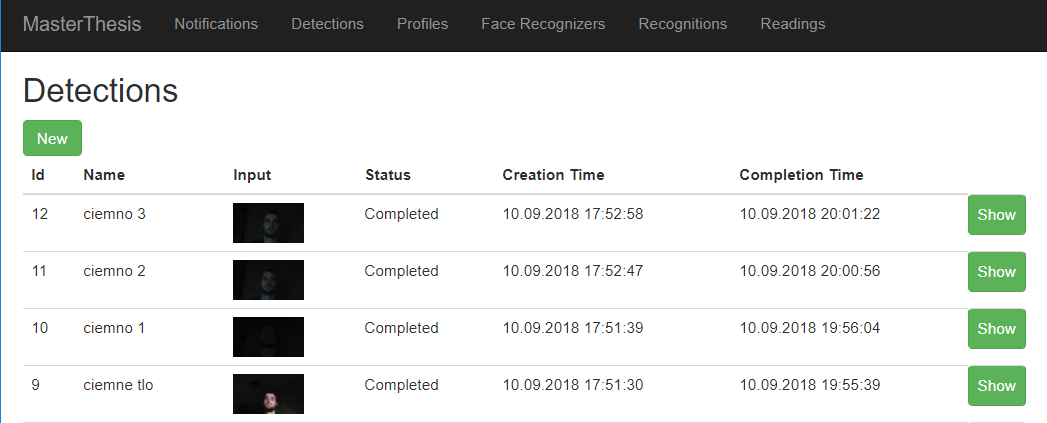
\includegraphics[scale=0.6]{detections.png}
	\caption{Widok detekcji twarzy}
	\label{fig:detections}
\end{figure}
Przycisk 'New' widoczny na \ref{fig:detections} pozwala na stworzenie nowego zadania wykrycia twarzy na obrazie, które zostanie przetworzone przez moduł aplikacji konsolowej. Na formularzu z rysunku \ref{fig:new_detection} należy podać nazwę zadania oraz za pomocą przycisku 'Wybierz plik' wybrać obraz w formacie png,jpg lub jpeg znajdujący się na dysku użytkownika.
\begin{figure}[H]
	\centering
	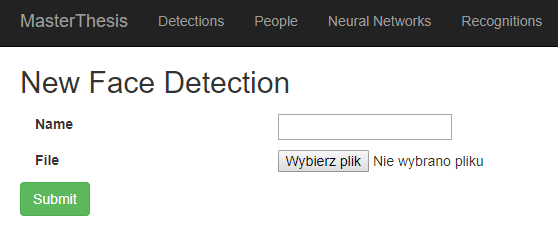
\includegraphics[scale=0.6]{new_detection.png}
	\caption{Tworzenie nowej detekcji}
	\label{fig:new_detection}
\end{figure}
Użycie przycisku 'Show' widocznego przy każdym zadaniu detekcji na rysunku \ref{fig:detections}, pozwoli na wyświetlenie szczegółów związanych z requestem, w tym wyników jeśli zadanie zostało zakończone.
\begin{figure}[H]
	\centering
	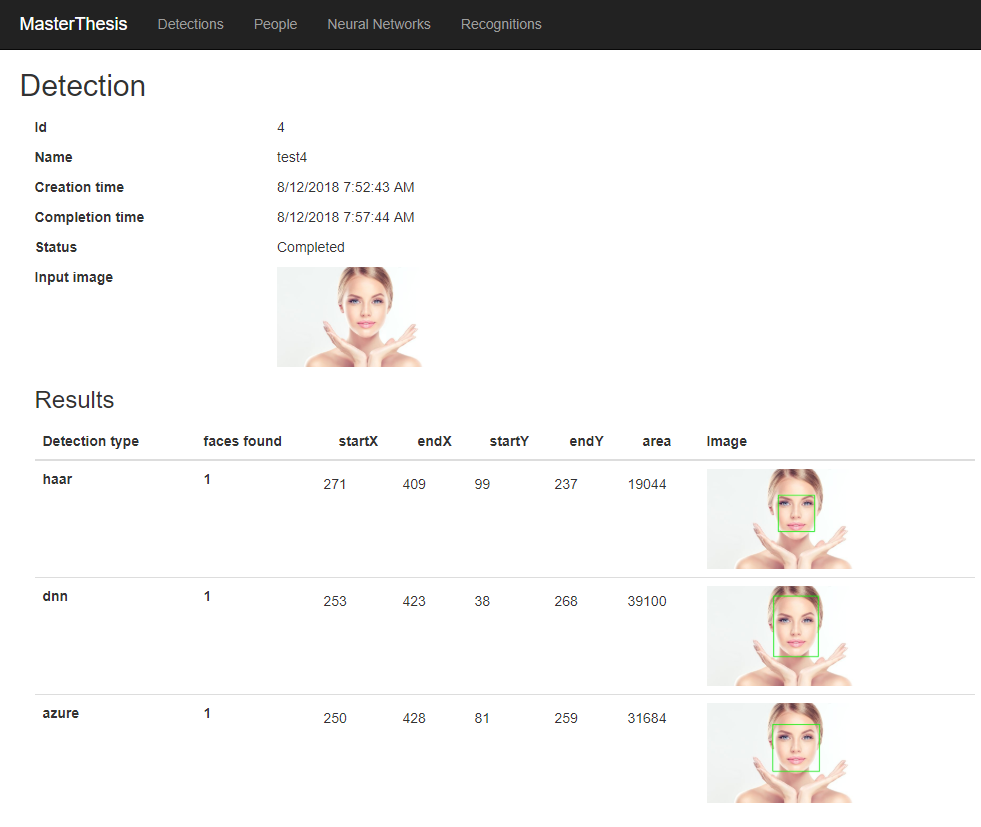
\includegraphics[scale=0.6]{detekcja_z_wynikami.png}
	\caption{Widok zakończonej detekcji}
	\label{fig:detekcja_zakonczona}
\end{figure}
Strona ze zdjęcia \ref{fig:detekcja_zakonczona} pozwala sprawdzić datę utworzenia oraz zakończenia zadania, obraz wejściowy, szczegółowe informacje o obszarze zidentyfikowanym jako twarz oraz sposobie jej wykrycia.
\subsection{People}
Strona 'People' służy do tworzenia nowych znanych tożsamości, które później mogą zostać wykorzystane jako dane uczące podczas trenowania sieci neuronowych. Do każdej osoby musi zostać przypisany zasób minimum 2 zdjęć. W przypadku braku możliwości wykrycia twarzy na zdjęciu, zostanie ono zignorowane podczas procesu nauczania.
\begin{figure}[H]
	\centering
	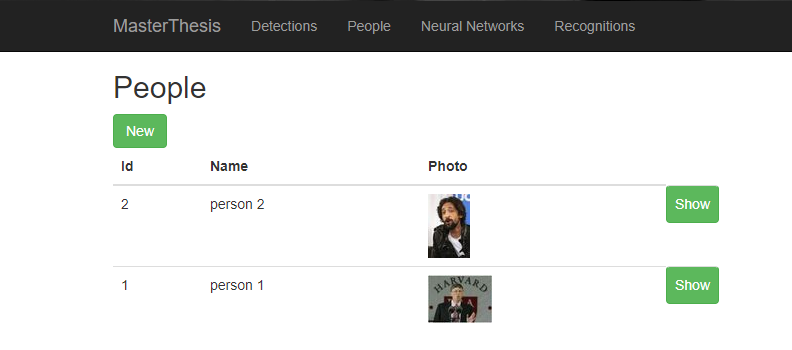
\includegraphics[scale=0.6]{people.png}
	\caption{Lista utworzonych ludzi}
	\label{fig:people}
\end{figure}
Nowa osoba może zostać utworzona w podobny sposób jak request detekcji twarzy. Jedyną różnicą jest wymóg wyboru kilku obrazów.
\begin{figure}[H]
	\centering
	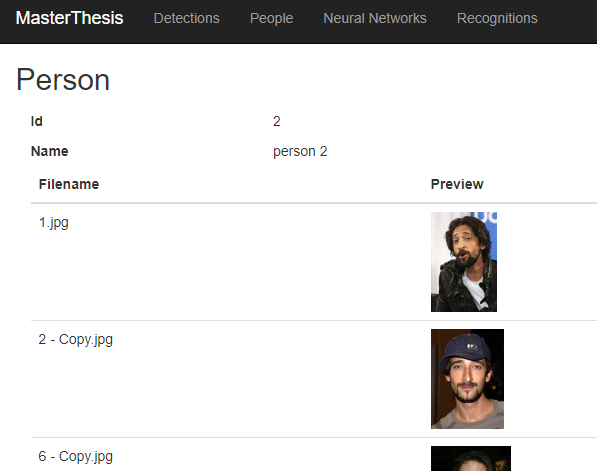
\includegraphics[scale=0.6]{person.png}
	\caption{Widok osoby}
	\label{fig:person}
\end{figure}
Utworzona osoba nie może być modyfikowana. Pierwsze załadowanie widoku osoby może trwać wydłużony czas z powodu procesu generowania linków do plików magazynowanych w usłudze Dropbox.

\subsection{Neural Networks}
\begin{figure}[H]
	\centering
	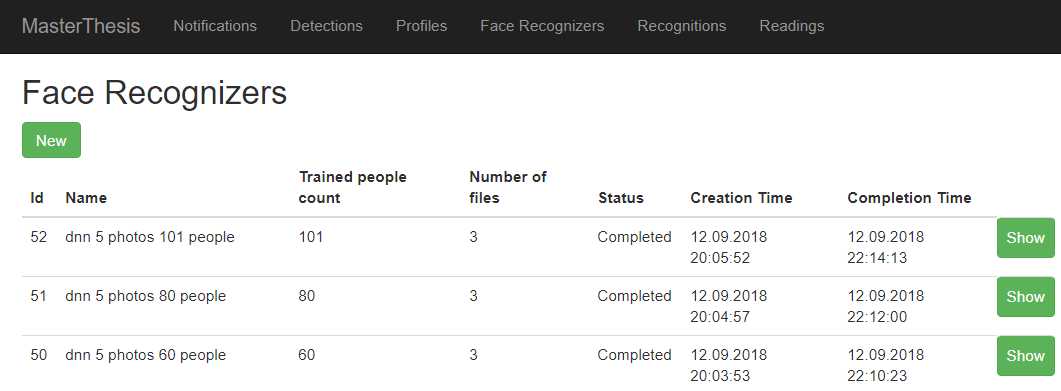
\includegraphics[scale=0.6]{neural_networks.png}
	\caption{Strona przedstawiająca istniejące grupy usług rozpoznawania tożsamości}
	\label{fig:sieci_neuronowe}
\end{figure}
W zakładce 'Neural Networks' użytkownik ma możliwość stworzenia grupy wybranych usług i sieci neuronowych, które zostaną nauczone rozpoznawać tożsamości utworzone w zakładce 'People'.
\begin{figure}[H]
	\centering
	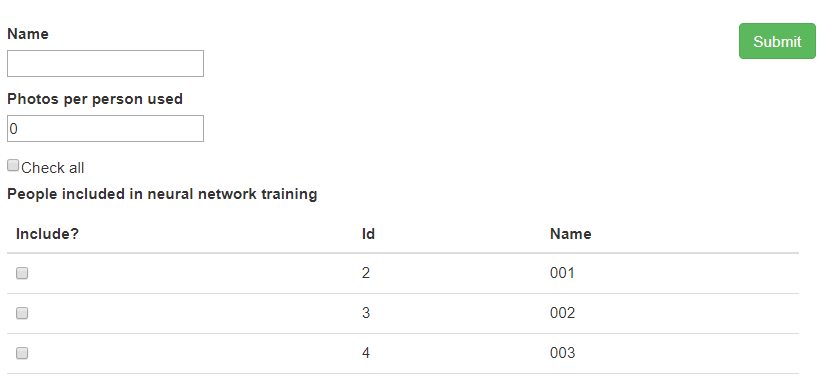
\includegraphics[scale=0.6]{nowa_siec.png}
	\caption{Tworzenie nowej grupy sieci neuronowych}
	\label{fig:nowa_siec}
\end{figure}
Każda istniejąca osoba zostanie wyświetlona jako checkbox, który należy zaznaczyć jeśli użytkownik chce by dana osoba została wykorzystana podczas procesu trenowania. Należy wybrać minimum 2 osoby, w przypadku wyboru mniejszej ilości osób, użytkownik zostanie poinformowany o tej konieczności.

Widok ukazany na rysunku \ref{fig:sieci_neuronowe} pozwala sprawdzić ile osób zostało użytych w procesie nauki oraz ile sieci neuronowych zostało utworzonych. Wyświetlenie jednej z grup pozwoli na uzyskanie bardziej szczegółowych informacji na temat wykorzystanych osób i utworzonych sieci, patrz rysunek \ref{fig:siec_neuronowa}.
\begin{figure}[H]
	\centering
	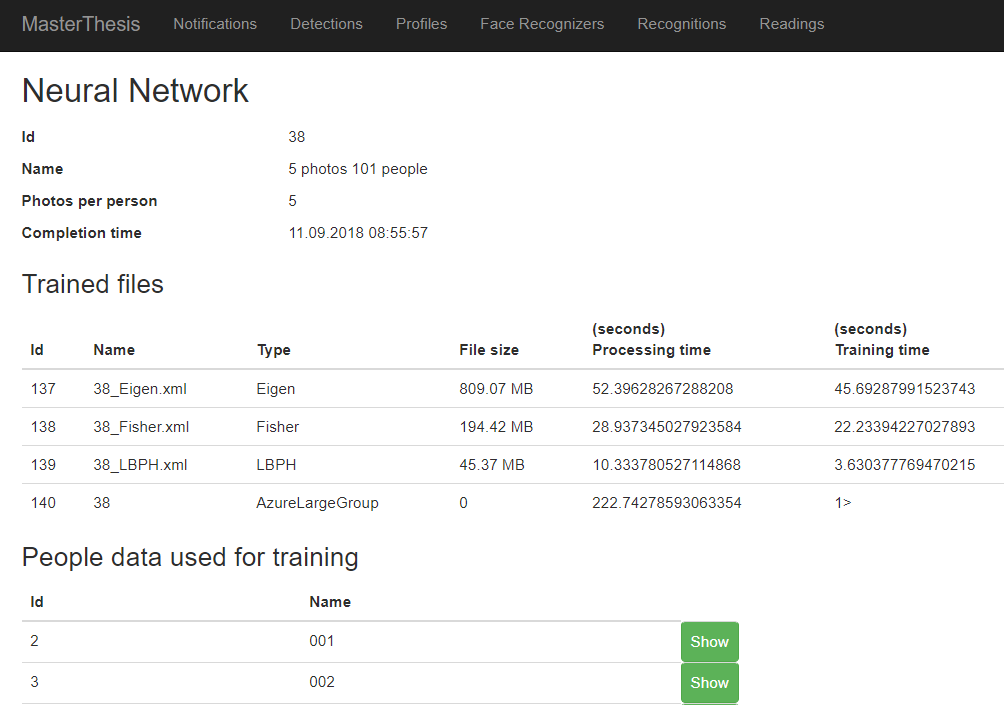
\includegraphics[scale=0.6]{siec_neuronowa.png}
	\caption{Szczegółowe informacje o grupie sieci neuronowych}
	\label{fig:siec_neuronowa}
\end{figure}

\subsection{Recognitions}
W sekcji 'Recognitions' użytkownik ma możliwość wykorzystać wcześniej utworzone zbiory sieci neuronowych w celu identyfikacji tożsamości na zdjęciu przedstawiającym pojedynczą osobę.
\begin{figure}[H]
	\centering
	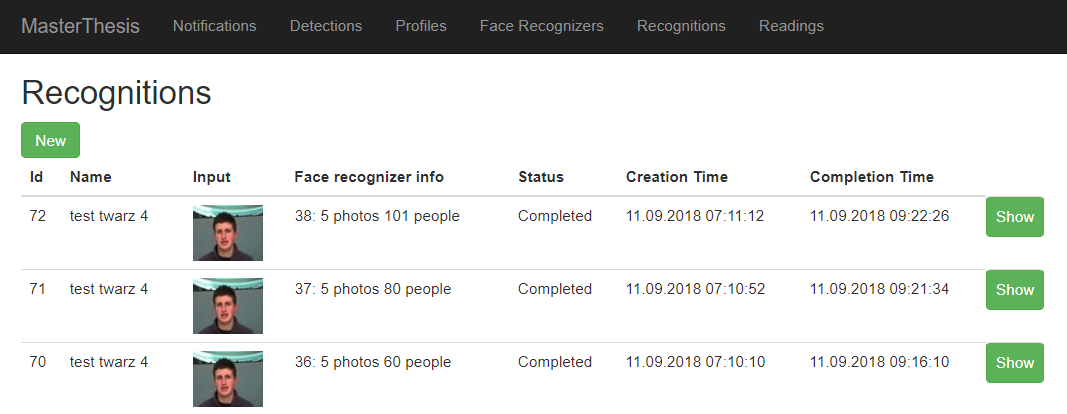
\includegraphics[scale=0.6]{recognitions.png}
	\caption{Lista zadań identyfikacji osoby}
	\label{fig:recognitions}
\end{figure}
Podobnie jak na pozostałych stronach, podczas tworzenia nowego zadania użytkownik będzie musiał uzupełnić prosty formularz. W formularzu przedstawionym na rysunku \ref{fig:new_recognition} należy załączyć jedno zdjęcie oraz wybrać grupę sieci neuronowych, która ma zostać wykorzystana do identyfikacji tożsamości osoby.
\begin{figure}[H]
	\centering
	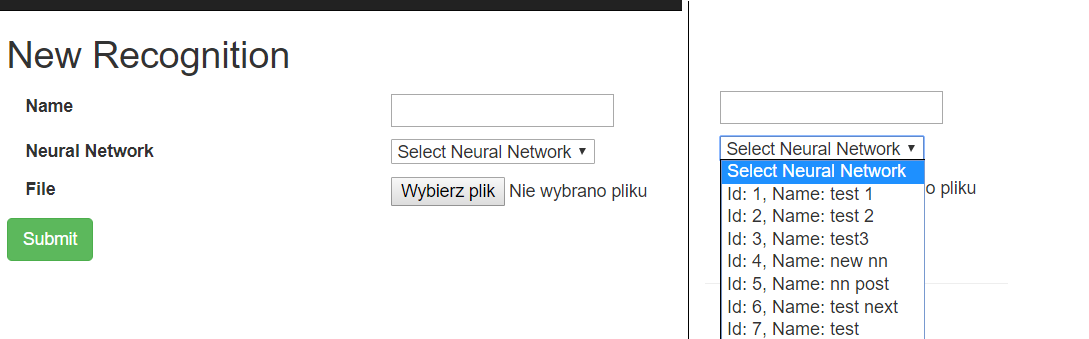
\includegraphics[scale=0.6]{new_recognition.png}
	\caption{Formularz tworzenia zadania identyfikacji}
	\label{fig:new_recognition}
\end{figure}
Po zakończonym procesie identyfikacji opisanym w kolejnym podrozdziale, użytkownik może wyświetlić wynik uzyskany przez każdą sieć dostępną w grupie. Przykładowy rezultat widoczny jest na zdjęciu \ref{fig:recognition}.
\begin{figure}[H]
	\centering
	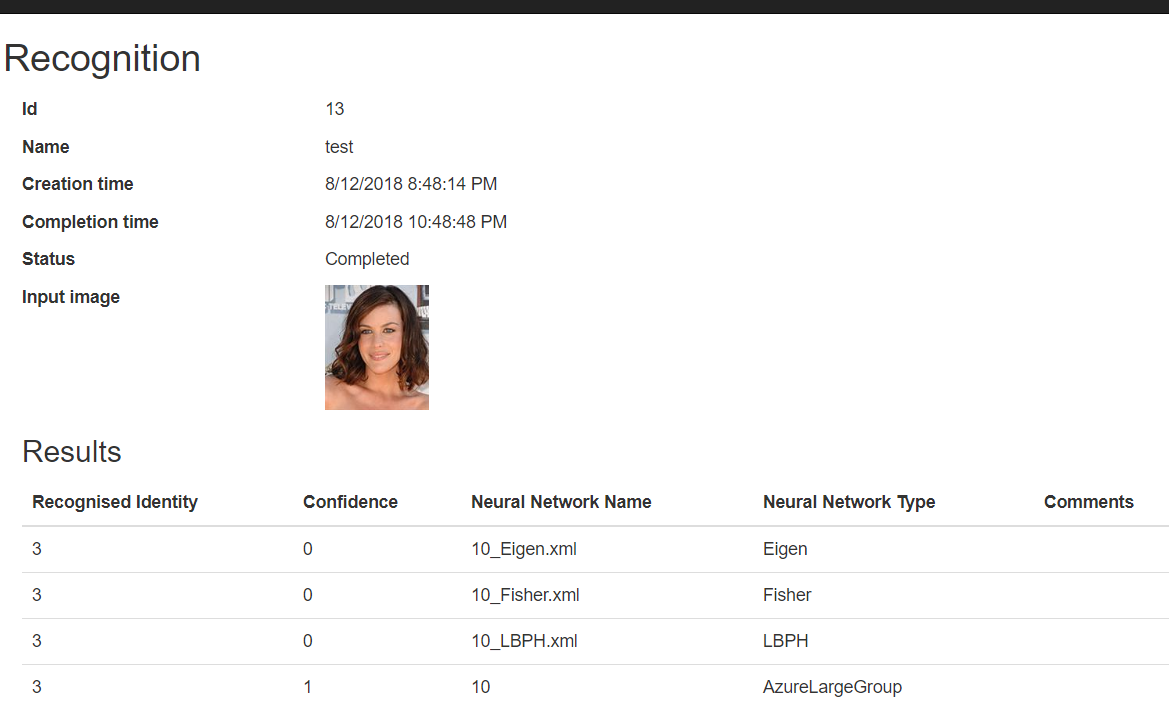
\includegraphics[scale=0.6]{recognition.png}
	\caption{Zakończony request identyfikacji}
	\label{fig:recognition}
\end{figure}

\section{Aplikacja konsolowa}
Aplikacja konsolowa powstała w celu przetwarzania czasochłonnych zadań w tle, tak by użytkownik aplikacji webowej nie doświadczał długich czasów ładowania oraz ewentualnych błędów podczas przerwania sesji lub połączenia internetowego ze stroną. Aplikacja konsolowa uruchamiana jest co 5 minut i przetwarza zadania trzech typów w kolejności widocznej na rysunku \ref{fig:worker_proces}. Poszczególne procesy zostały szerzej opisane w kolejnych podrozdziałach.
\begin{figure}[H]
	\centering
	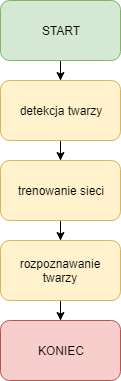
\includegraphics[scale=0.6]{worker_proces.png}
	\caption{Proces działania aplikacji konsolowej}
	\label{fig:worker_proces}
\end{figure}



\subsection{Technologie}


\subsection{Proces wykrywania twarzy}
Uogólniony proces detekcji twarzy na obrazie został przedstawiony na grafie \ref{fig:wykrywanie_proces}. Szczegółowy proces dla każdej z metod detekcji przedstawiono w rozdziale \ref{detekcja_twarzy}.
\begin{figure}[H]
	\centering
	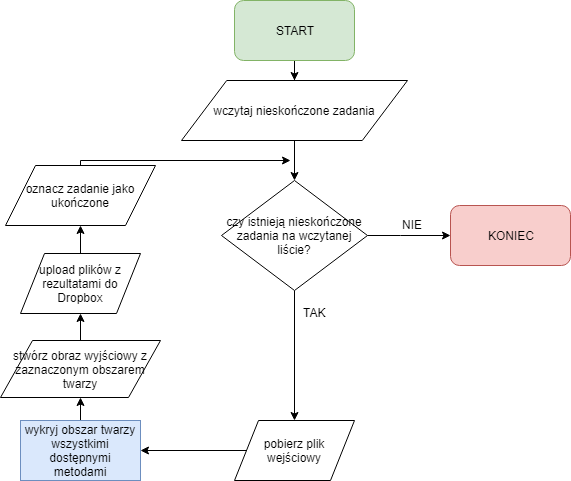
\includegraphics[scale=0.6]{wykrywanie_twarzy.png}
	\caption{Proces wykrywania twarzy}
	\label{fig:wykrywanie_proces}
\end{figure}

\subsection{Proces trenowania sieci neuronowych}
Proces trenowania sieci został przedstawiony na grafie \ref{fig:trenowanie_proces}, szczegółowe informacje o przygotowaniu danych uczących i procesie nauczania zostały opisane w kolejnej sekcji.
\begin{figure}[H]
	\centering
	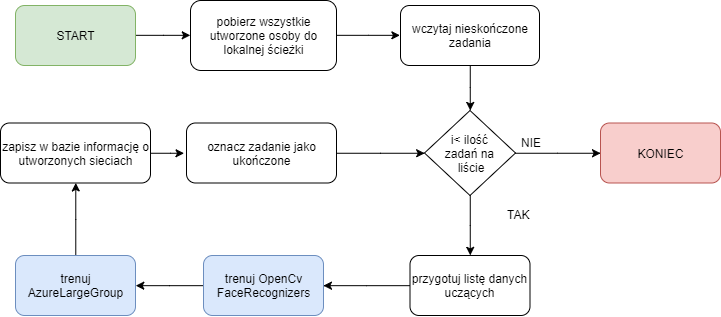
\includegraphics[scale=0.6]{proces_nauczania.png}
	\caption{Proces trenowania sieci}
	\label{fig:trenowanie_proces}
\end{figure}

\subsubsection{Przygotowanie danych trenujących} \label{przygotowanie_danych_uczących}

\subsubsection{Trenowanie sieci} \label{trenowanie_sieci}

\subsection{Proces rozpoznawania twarzy}


\section{Program zarządzający domem}

%%%%%%%%%%%%%%%%%%%%%%%%	Aplikacja internetowa
\chapter{Aplikacja internetowa}
Aplikacja webowa jest jedyną częścią systemu, do której użytkownik może mieć bezpośredni dostęp. Strona powstała w celu maksymalnego uproszczenia procesu badania kolejnych algorytmów i usług, które różniły się sposobem podawania danych wejściowych, sposobem uczenia oraz formatem zwracanych odpowiedzi. Do pozostałych zalet takiego rozwiązania należy ułatwienie przechowywania danych, poprzez umieszczenie ich we wspólnym miejscu co pomaga, w późniejszej interpretacji wyników.
\begin{figure}[H]
	\centering
	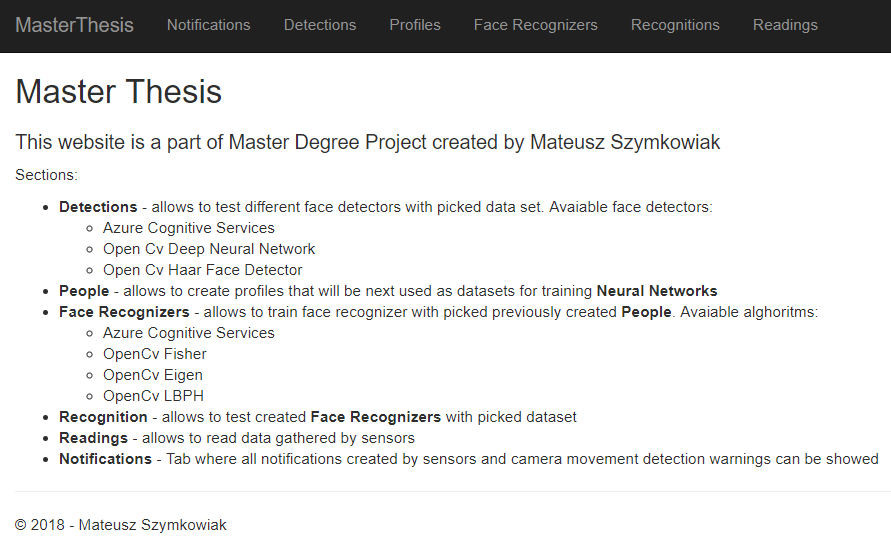
\includegraphics[scale=0.7]{aplikacja_webowa_razor_widok.png}
	\caption{Wygląd strony głównej}
	\label{fig:strona_glowna_razor}
\end{figure}
Zgodnie z interfejsem przedstawionym na rysunku \ref{fig:strona_glowna_razor}, strona została podzielona na 5 głównych sekcji:
\begin{itemize}
\item Detections- detekcje,
\item People- ludzie,
\item Neural Networks- sieci neuronowe,
\item Recognition- rozpoznawanie,
\item Sensor Readings- odczyty sensorów.
\end{itemize}

\section{Technologie}
Aplikacja webowa powstała w najnowszej kompilacji .NET Core 2, będącej międzyplatformową strukturą open source o wysokiej wydajności służącą do tworzenia nowoczesnych aplikacji internetowych opartych na usługach chmurowych. Logika biznesowa aplikacji została zaprogramowana w języku C\#. Warstwa widoku powstała w dwóch dostępnych rozwiązaniach, nieznacznie różniących się wyglądem, ale znacznie odbiegających od siebie sposobem działania. Przed omówieniem poszczególnych rozwiązań przedstawiono, krótkie definicje wykorzystanego wzorca projektowego MVC oraz technologii SPA. 

\subsection{Rozwiązanie 1- Razor Pages}
Pierwsza wersja została oparta o strony tworzone w technologi Razor Pages opartej o składnię Razor oraz podstawowe technologie webowe: HTML i CSS. Taki sposób tworzenia warstwy prezentacji jest zalecany dla aplikacji .NET Core, ponieważ pozwala zminimalizować ilość pracy wymaganej na jej utworzenie oraz zapewnia bardzo prosty proces wdrożenia. Aplikacja utworzona z pomocą Razor'a została zaprezentowana na rysunku \ref{fig:strona_glowna_razor}.

\subsection{Rozwiązanie 2- Angular 4}
Druga wersja widoku aplikacji oferuje dostęp do tych samych możliwości co pierwsze rozwiązanie, ale powstała przy pomocy frameworka webowego- Angular 4. Strona główna widoczna jest na rysunku \ref{fig:strona_glowna_angular}. Angular jest open sourcowym frameworkiem używanym do tworzenia aplikacji SPA (Single Page Application), napisany w języku TypeScript i wspierany oraz rozwijany przez Google.
\begin{figure}[H]
	\centering
	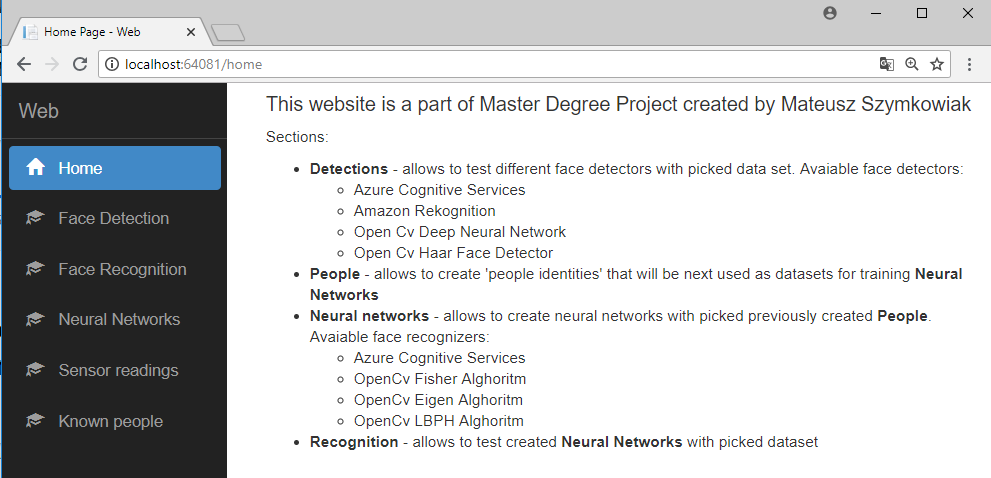
\includegraphics[scale=0.6]{aplikacja_webowa_angular_widok.png}
	\caption{Strona główna widoku utworzonym w Angular 4}
	\label{fig:strona_glowna_angular}
\end{figure}

\section{Detections}
Detections jest stroną odpowiedzialną za wykrywanie twarzy na obrazach przesłanych do systemu. Na głównej stronie możemy zobaczyć wszystkie zlecone detekcje, zarówno nowe jak i już zakończone.
\begin{figure}[H]
	\centering
	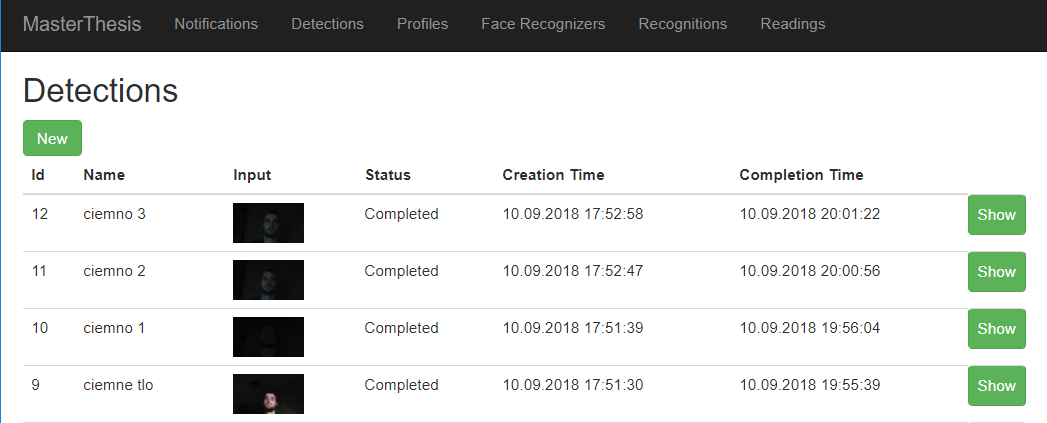
\includegraphics[scale=0.6]{detections.png}
	\caption{Widok detekcji twarzy}
	\label{fig:detections}
\end{figure}
Przycisk 'New' widoczny na \ref{fig:detections} pozwala na stworzenie nowego zadania wykrycia twarzy na obrazie, które zostanie przetworzone przez moduł aplikacji konsolowej. Na formularzu z rysunku \ref{fig:new_detection} należy podać nazwę zadania oraz za pomocą przycisku 'Wybierz plik' wybrać obraz w formacie png,jpg lub jpeg znajdujący się na dysku użytkownika.
\begin{figure}[H]
	\centering
	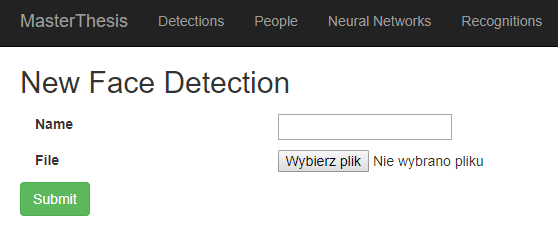
\includegraphics[scale=0.6]{new_detection.png}
	\caption{Tworzenie nowej detekcji}
	\label{fig:new_detection}
\end{figure}
Użycie przycisku 'Show' widocznego przy każdym zadaniu detekcji na rysunku \ref{fig:detections}, pozwoli na wyświetlenie szczegółów związanych z requestem, w tym wyników jeśli zadanie zostało zakończone.
\begin{figure}[H]
	\centering
	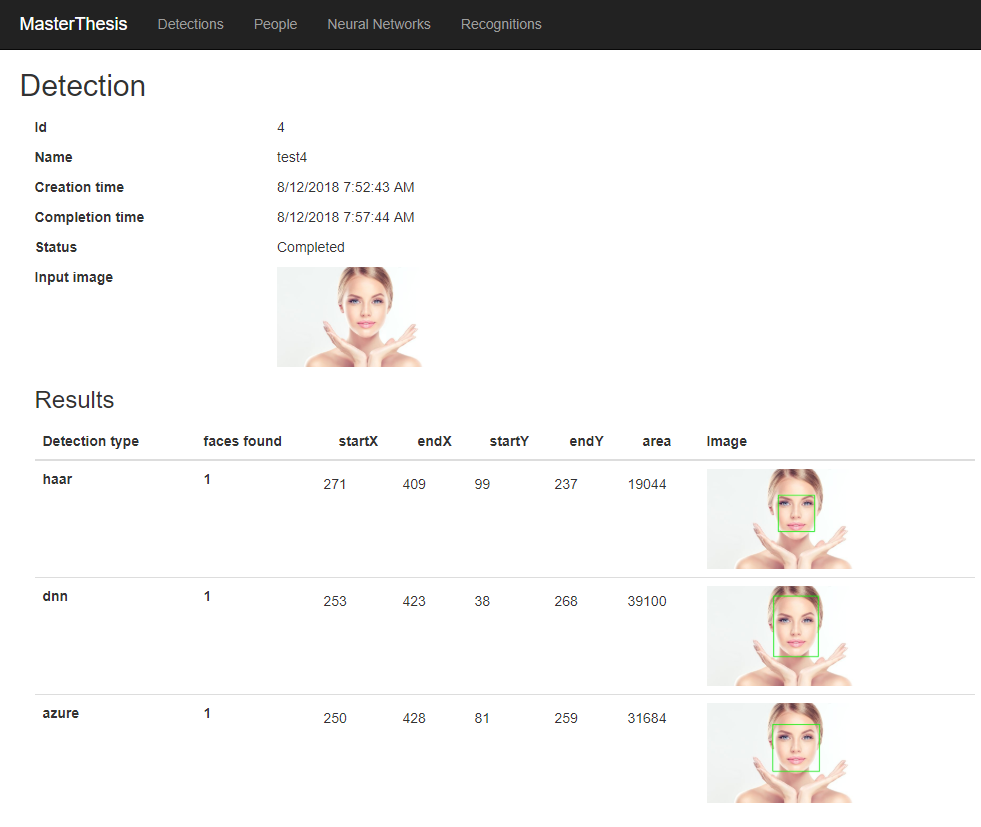
\includegraphics[scale=0.6]{detekcja_z_wynikami.png}
	\caption{Widok zakończonej detekcji}
	\label{fig:detekcja_zakonczona}
\end{figure}
Strona ze zdjęcia \ref{fig:detekcja_zakonczona} pozwala sprawdzić datę utworzenia oraz zakończenia zadania, obraz wejściowy, szczegółowe informacje o obszarze zidentyfikowanym jako twarz oraz sposobie jej wykrycia.
\section{People}
Strona 'People' służy do tworzenia nowych znanych tożsamości, które później mogą zostać wykorzystane jako dane uczące podczas trenowania sieci neuronowych. Do każdej osoby musi zostać przypisany zasób minimum 2 zdjęć. W przypadku braku możliwości wykrycia twarzy na zdjęciu, zostanie ono zignorowane podczas procesu nauczania.
\begin{figure}[H]
	\centering
	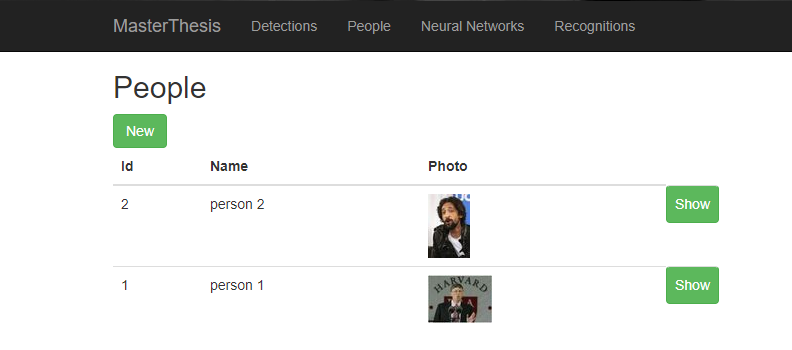
\includegraphics[scale=0.6]{people.png}
	\caption{Lista utworzonych ludzi}
	\label{fig:people}
\end{figure}
Nowa osoba może zostać utworzona w podobny sposób jak request detekcji twarzy. Jedyną różnicą jest wymóg wyboru kilku obrazów.
\begin{figure}[H]
	\centering
	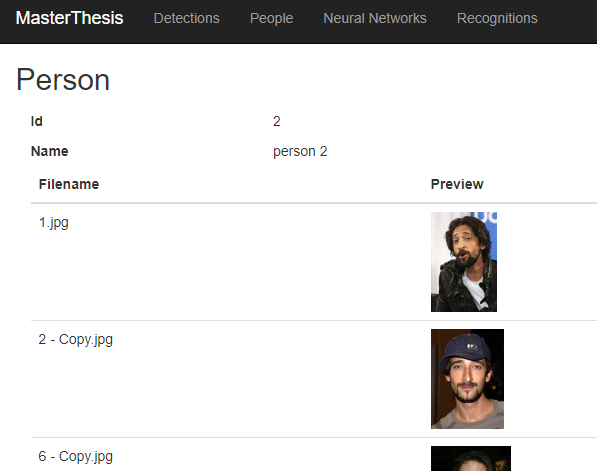
\includegraphics[scale=0.6]{person.png}
	\caption{Widok osoby}
	\label{fig:person}
\end{figure}
Utworzona osoba nie może być modyfikowana. Pierwsze załadowanie widoku osoby może trwać wydłużony czas z powodu procesu generowania linków do plików magazynowanych w usłudze Dropbox.

\section{Neural Networks}
\begin{figure}[H]
	\centering
	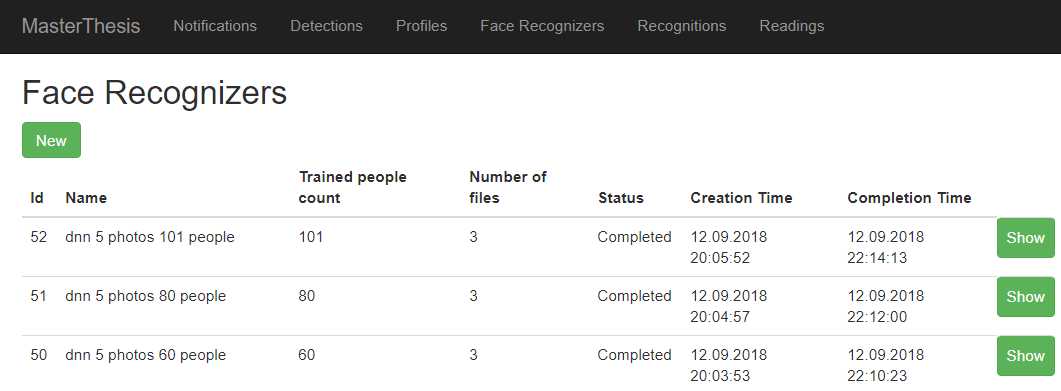
\includegraphics[scale=0.6]{neural_networks.png}
	\caption{Strona przedstawiająca istniejące grupy usług rozpoznawania tożsamości}
	\label{fig:sieci_neuronowe}
\end{figure}
W zakładce 'Neural Networks' użytkownik ma możliwość stworzenia grupy wybranych usług i sieci neuronowych, które zostaną nauczone rozpoznawać tożsamości utworzone w zakładce 'People'.
\begin{figure}[H]
	\centering
	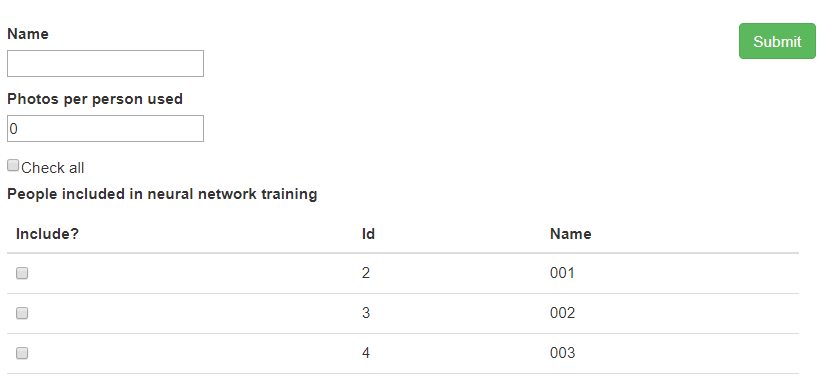
\includegraphics[scale=0.6]{nowa_siec.png}
	\caption{Tworzenie nowej grupy sieci neuronowych}
	\label{fig:nowa_siec}
\end{figure}
Każda istniejąca osoba zostanie wyświetlona jako checkbox, który należy zaznaczyć jeśli użytkownik chce by dana osoba została wykorzystana podczas procesu trenowania. Należy wybrać minimum 2 osoby, w przypadku wyboru mniejszej ilości osób, użytkownik zostanie poinformowany o tej konieczności.

Widok ukazany na rysunku \ref{fig:sieci_neuronowe} pozwala sprawdzić ile osób zostało użytych w procesie nauki oraz ile sieci neuronowych zostało utworzonych. Wyświetlenie jednej z grup pozwoli na uzyskanie bardziej szczegółowych informacji na temat wykorzystanych osób i utworzonych sieci, patrz rysunek \ref{fig:siec_neuronowa}.
\begin{figure}[H]
	\centering
	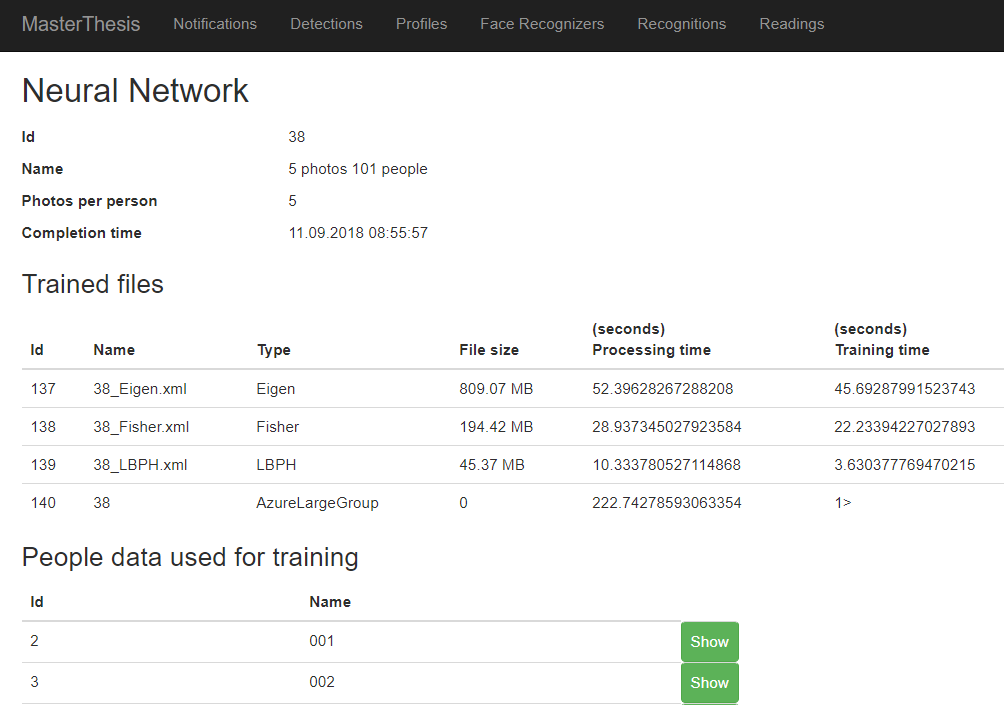
\includegraphics[scale=0.6]{siec_neuronowa.png}
	\caption{Szczegółowe informacje o grupie sieci neuronowych}
	\label{fig:siec_neuronowa}
\end{figure}

\section{Recognitions}
W sekcji 'Recognitions' użytkownik ma możliwość wykorzystać wcześniej utworzone zbiory sieci neuronowych w celu identyfikacji tożsamości na zdjęciu przedstawiającym pojedynczą osobę.
\begin{figure}[H]
	\centering
	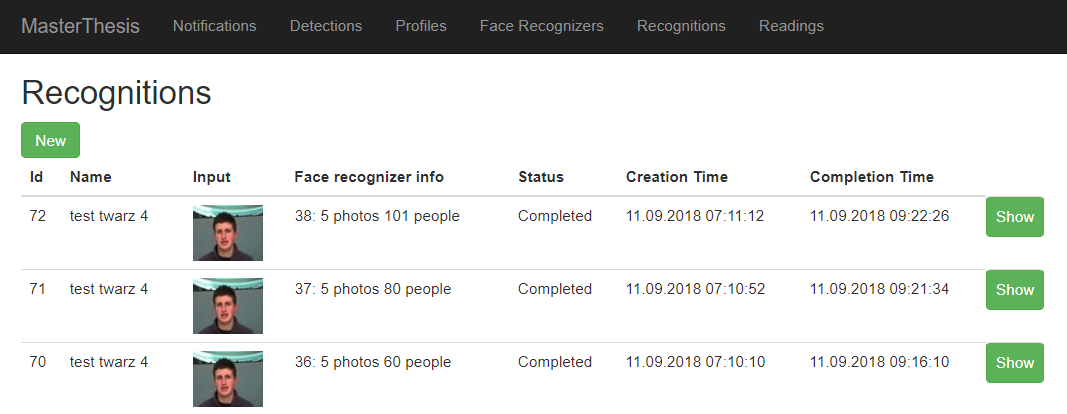
\includegraphics[scale=0.6]{recognitions.png}
	\caption{Lista zadań identyfikacji osoby}
	\label{fig:recognitions}
\end{figure}
Podobnie jak na pozostałych stronach, podczas tworzenia nowego zadania użytkownik będzie musiał uzupełnić prosty formularz. W formularzu przedstawionym na rysunku \ref{fig:new_recognition} należy załączyć jedno zdjęcie oraz wybrać grupę sieci neuronowych, która ma zostać wykorzystana do identyfikacji tożsamości osoby.
\begin{figure}[H]
	\centering
	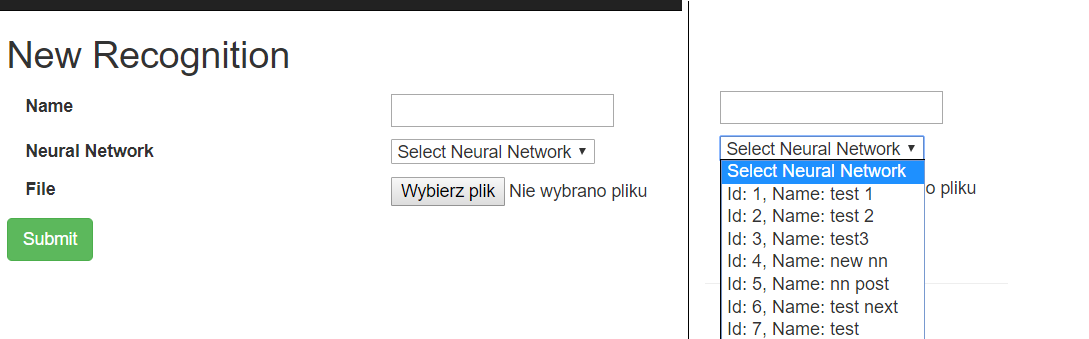
\includegraphics[scale=0.6]{new_recognition.png}
	\caption{Formularz tworzenia zadania identyfikacji}
	\label{fig:new_recognition}
\end{figure}
Po zakończonym procesie identyfikacji opisanym w kolejnym podrozdziale, użytkownik może wyświetlić wynik uzyskany przez każdą sieć dostępną w grupie. Przykładowy rezultat widoczny jest na zdjęciu \ref{fig:recognition}.
\begin{figure}[H]
	\centering
	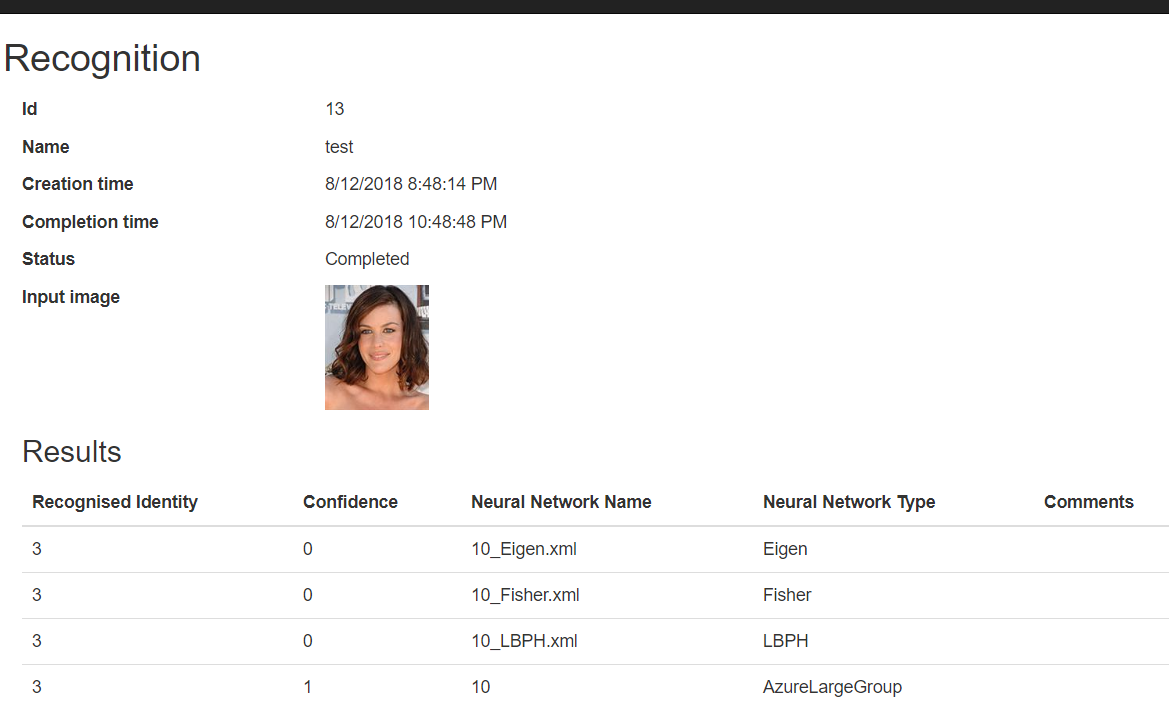
\includegraphics[scale=0.6]{recognition.png}
	\caption{Zakończony request identyfikacji}
	\label{fig:recognition}
\end{figure}

\section{Readings \textcolor{red}{TODO}}
\textcolor{red}{zrobić zdjęcia i opisać}

\section{Notifications \textcolor{red}{TODO}}
\textcolor{red}{zrobić zdjęcia i opisać}

%%%%%%%%%%%%%%%%%%%%%%%%	Aplikacja konsolowa
1\chapter{Aplikacja konsolowa}
Aplikacja konsolowa powstała w celu przetwarzania czasochłonnych zadań w tle, tak by użytkownik aplikacji webowej nie doświadczał długich czasów ładowania oraz ewentualnych błędów podczas przerwania sesji lub połączenia internetowego ze stroną. Aplikacja konsolowa uruchamiana jest co 5 minut i przetwarza zadania trzech typów w kolejności widocznej na rysunku \ref{fig:worker_proces}. Poszczególne procesy zostały szerzej opisane w kolejnych podrozdziałach.
\begin{figure}[H]
	\centering
	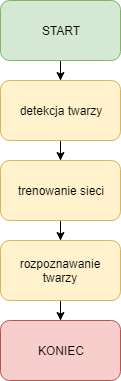
\includegraphics[scale=0.6]{worker_proces.png}
	\caption{Proces działania aplikacji konsolowej}
	\label{fig:worker_proces}
\end{figure}

\section{Technologie}
Aplikacja konsolowa powstała w języku programowania Python w wersji trzeciej. W początkowej fazie projektu za wyborem tego języka przemawiała wieloplatformowość, możliwości wprowadzania szybkich zmian w kodzie i brak potrzeby go kompilowania. C\#, który został wybrany do stworzenia aplikacji webowej okazał się nie przystosowany do uruchomienia na platformie Raspberry Pi z powodu braku dostępnego .NET Core SDK na procesory ARM oraz wymaganiu znacznie większej ilości zasobów niż Python. Ostatecznie aplikacja konsolowa została przeniesiona na zewnętrzny serwer, ale popularność Pythona pozwoliła na szybką integrację z usługami firm trzecich, dzięki przygotowanym przez firmy paczki deweloperskie.

\section{Proces wykrywania twarzy}
Uogólniony proces detekcji twarzy na obrazie został przedstawiony na grafie \ref{fig:wykrywanie_proces}.
Proces przetwarzania zadań detekcji rozpoczyna się od pobrania z bazy wszystkich żądań o statusie 'New'. Następnie każde zadanie przetwarzane jest osobno. Dla aktualnie procesowanego zadania pobierany jest obraz wejściowy z usługi Dropbox i zapisywany w lokalnym folderze. Następnym krokiem jest wywołanie procesu odpowiedzialnego za odpowiednie przygotowanie zdjęcia, a następnie pozyskanie oczekiwanych wyników, w sposób odpowiedni dla danego sposobu. Krok ten został szerzej opisany w podrozdziałach \ref{detekcja_haar}, \ref{detekcja_dnn} i \ref{detekcja_azure}. po uzyskaniu wyników każdą dostępną w programie metodą, zostaje utworzony obraz wyjściowy dla każdej metody (haar, azure, ..), które zostaje wgrany do odpowiedniego folderu w usłudze Dropbox. Po poprawnym wgraniu plików wynikowych informacja o rezultatach zostaje dodana do bazy danych. Po wykonaniu zadania bez żadnych błędów, request zostaje oznaczony jako zakończony, w innym przypadku zostaje nadany mu status 'Error'. Proces powtarzany jest dla każdego wpisu pozyskanego z bazy.
\begin{figure}[H]
	\centering
	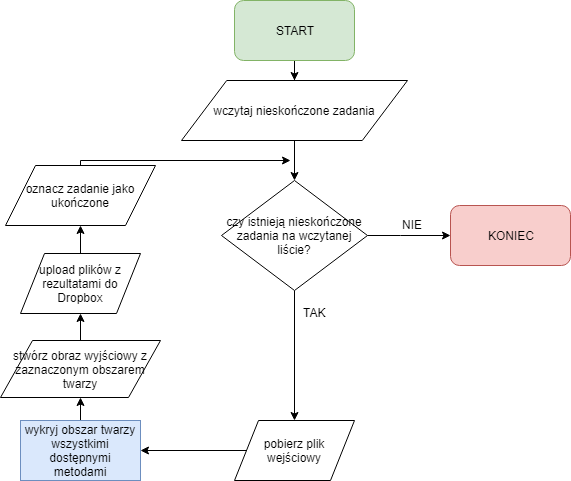
\includegraphics[scale=0.6]{wykrywanie_twarzy.png}
	\caption{Proces wykrywania twarzy}
	\label{fig:wykrywanie_proces}
\end{figure}

\subsection{Open Cv Haar} \label{detekcja_haar}
Pierwszą z metod detekcji twarz, która została zintegrowana z programem jest detekcja metodą Haar'a. Algorytm został opisany w rozdziale \ref{haar}. Przed uruchomieniem detekcji twarzy, obraz wejściowy należy odpowiednio przygotować. W tym celu wcześniej pobrany obraz zostaje wczytany do programu i przekonwertowany do odcieni szarości. Tak przygotowany obraz można poddać detekcji. Detektor zwraca współrzędne obszarów zawierających w sobie twarze. Tak uzyskane dane należy przekonwertować do formatu, który został przyjęty jako wspólny dla wszystkich metod.
\begin{figure}[H]
	\centering
	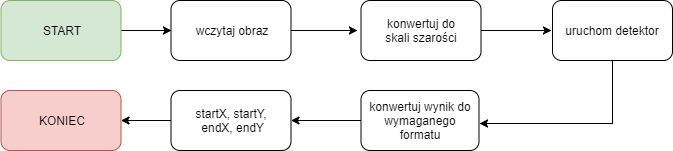
\includegraphics[scale=0.6]{detekcja_haar.png}
	\caption{Wykrywanie twarzy metodą Haar}
	\label{fig:wykrywanie_haar}
\end{figure}

\subsection{Open Cv Dnn} \label{detekcja_dnn}
Proces detekcji z wykorzystaniem głęboko uczonej sieci neuronowej nie wymaga formatowania obrazu do skali szarości, ale za to obraz musi zostać przeskalowany do odpowiedniego, wcześniej przyjętego rozmiaru. Dodatkową zaletą tej metody jest format odpowiedzi detektora, który oprócz obszaru zawierającego twarz zwraca również 'pewność' z jaką twarz została wykryta, co pozwala na odfiltrowanie niezadowalających użytkownika wyników.
\begin{figure}[H]
	\centering
	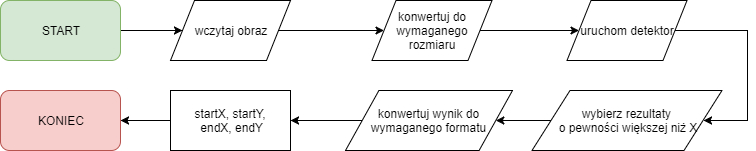
\includegraphics[scale=0.6]{detekcja_dnn.png}
	\caption{Wykrywanie twarzy metodą DNN}
	\label{fig:wykrywanie_dnn}
\end{figure}

\subsection{Azure Cognitive Services} \label{detekcja_azure}
Kolejna wykorzystana metoda detekcji twarzy, korzysta z usługi dostępnej na platformie Azure, dzięki czemu środowisko rozruchowe zostaje odciążone z obliczeń związanych z przetwarzaniem obrazu. Proces wykrycia twarzy ogranicza się do przesłania wybranego obrazu do Cognitive Services Api. W odpowiedzi klient uzyskuje JSON zawierający parametry, które podano jako wymagane podczas wykonywania zapytania. JSON zostaje zparsowany na obiekt, którego wartości zostają przekonwertowane do wymaganego formatu [startX, startY, endX, endY].
\begin{figure}[H]
	\centering
	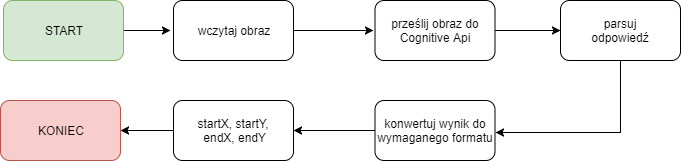
\includegraphics[scale=0.6]{detekcja_azure.png}
	\caption{Wykrywanie twarzy używając Azure Cognitive Services}
	\label{fig:wykrywanie_azure}
\end{figure}


\section{Proces trenowania sieci neuronowych}
\begin{figure}[H]
	\centering
	\includegraphics[scale=0.6]{proces_nauczania.png}
	\caption{Proces trenowania sieci}
	\label{fig:trenowanie_proces}
\end{figure}
Proces trenowania sieci został przedstawiony na grafie \ref{fig:trenowanie_proces}. Proces zaczyna się od sprawdzenia jakie dane uczące (osoby utworzone w zakładce 'People' aplikacji webowej) są dostępne lokalnie. Repozytorium zostaje porównane z danymi dostępny w bazie, a następnie zostają pobrane zdjęcia wszytskich brakujących osób do lokalnej ścieżki. Kolejnym krokiem jest pobrania z bazy wszystkich nowych grup sieci neuronowych, które nie zostały jeszcze zakończone. Następnie dla każdego zgłoszenia z listy wykonywany jest proces przygotowania danych uczących na podstawie zdjęć osób, które wybrano podczas tworzenia sieci neuronowej w aplikacji webowej. Po odpowiednim przygotowaniu danych sieć zostaje nauczona i dla większości metod zostaje utworzony plik w formacie xml przechowujący wytrenowany model. Taki plik zostaje dodany do bazy oraz wysłany do odpowiedniego folderu w Dropboxie. W przypadku braku komplikacji, request zostaje oznaczony jako zakończony. Proces zostaje powtórzony dla każdego zadania wczytanego do listy na początku grafu. Sposób przygotowania danych oraz nauczania dla poszczególnych metod został opisany w kolejnych podrozdziałach.

\subsection{Trenowanie identyfikatorów Open Cv} \label{trenowanie_open_cv}
\begin{figure}[H]
	\centering
	\includegraphics[scale=0.6]{trenowanie_open_cv.png}
	\caption{Trenowanie sieci neuronowej Open Cv}
	\label{fig:trenowanie_open_cv}
\end{figure}
Ogólny schemat procesu trenowania identyfikatorów twarzy OpenCv (Eigenfaces, Fisherfaces, LHGP) został przedstawiony na rysunku \ref{fig:trenowanie_open_cv}. Proces rozpoczyna się od stworzenia listy zawierającej wszystkie przypisane do sieci osoby oraz załączone do nich obrazy. Następnie dla każdego zdjęcia z listy zostaje wykonany preprocessing. Pierwszym krokiem jest próba wykrycia twarzy na obrazie. W przypadku nie znalezienia twarzy, obraz zostaje zignorowany i program przechodzi do przetwarzania kolejnego obrazu. Jeśli na zdjęciu zostanie zlokalizowana twarz, to obszar ją zawierający zostaje przeskalowany do odcieni szarości, a następnie przekonwertowany do postaci numpy array. Wektor zawierający informację o obrazie twarzy zostaje dodany do listy uczącej wraz z odpowiadającym mu ID osoby, od której pochodził obraz. Po przetworzeniu wszystkich obrazów na liście, zostaje utworzony jeden z trzech wcześniej wymienionych identyfikatorów twarzy. Ostatnim krokiem jest wywołanie funkcji uczącej.

\subsection{Trenowanie identyfikatora Azure} \label{trenowanie_azure}
\begin{figure}[H]
	\centering
	\includegraphics[scale=0.55]{trenowanie_azure.png}
	\caption{[DO POPRAWY] Trenowanie usługi Azure Cognitive Services}
	\label{fig:trenowanie_azure}
\end{figure}
Proces rozpoczyna się od wczytania wszystkich osób oraz ich zdjęć, które zostały przypisane do zadania trenowania sieci. Na diagramie \ref{fig:trenowanie_azure} niebieskim kolorem oznaczono zapytania do Azure Cognitive Services Api. Pierwszym i najważniejszym krokiem jest utworzenie nowej AzureLargeGroup, do której w następnym kroku zostaną dodane id/nazwy wszystkich osób znajdujących się na wczytanej liście.  Następnie każdy obraz z listy zostaje przypisany odpowiedniej osobie w AzureLargeGroup. W tym rozwiązaniu klient nie musi martwić się detekcją twarzy na obrazie, bo jest ona wykonywana przez usługę Azure po przesłaniu obrazu. W przypadku problemów z wykryciem twarzy na obrazie, zostanie zwrócona informacja mówiąca o tym że plik zostanie zignorowany podczas procesu nauczania. Po dodaniu wszystkich zdjęć, program wywołuje funkcję trenowania nowej sieci na podstawie danych dołączonych do AzureLargeGroup. Już po kilku sekundach, identyfikator tożsamości udostępniony przez usługę Azure jest gotowy do działania.

\section{Proces rozpoznawania twarzy}
\begin{figure}[H]
	\centering
	\includegraphics[scale=0.6]{rozpoznawanie_twarzy.png}
	\caption{Proces identyfikacji tożsamości}
	\label{fig:rozpoznawanie_proces}
\end{figure}

\subsection{OpenCv}
\begin{figure}[H]
	\centering
	\includegraphics[scale=0.6]{rozpoznawanie_open_cv.png}
	\caption{Proces identyfikacji osoby wykorzystując Open Cv}
	\label{fig:rozpoznawanie_open_cv}
\end{figure}

\subsection{Azure Cognitive Services}
\begin{figure}[H]
	\centering
	\includegraphics[scale=0.6]{rozpoznawanie_azure.png}
	\caption{Proces identyfikacji osoby wykorzystując Azure Cognitive Servces}
	\label{fig:rozpoznawanie_azure}
\end{figure}

%%%%%%%%%%%%%%%%%%%%%%%%	Aplikacja konsolowa
\chapter{Aplikacja konsolowa do zarządzania domem} \label{aplikacja_zarzadzanie}
Aplikacja konsolowa do zarządzania domem służy jako aplikacja odpowiedzialna za wszystkie działania związane z Raspberry Pi oraz jego peryferiami. Na te zadania składają się 2 czynności:
\begin{itemize}
\item odczyt wartości sensorów,
\item detekcja ruchu.
\end{itemize}
Obie czynności wykonywane są niezależnie od siebie. Funkcja wykrywania ruchu działa bez przerwy, w przypadku problemu zostanie ponownie uruchomiona po około minucie za pomocą zadania wpisanego do serwisu Crontab. Odczyt parametrów wskazywanych przez czujniki odbywa się cyklicznie co 1 minutę.

\section{Odczyt wartości sensorów}
\begin{figure}[H]
	\centering
	\includegraphics[scale=0.6]{odczyt_czujnikow.png}
	\caption{Proces pobierania danych z sensorów}
	\label{fig:wykrywanie_proces}
\end{figure}
Proces zbierania danych z sensorów rozpoczyna się od pobrania odczytów z czujnika DHT11. Raspberry komunikuje się z czujnikiem za pomocą protokołu 1-wire. Do pobrania wartości wykorzystano bibliotekę dedykowaną dla tego czujnika i języka Python. Po prawidłowym odczycie, każdy z parametrów (temperatura i wilgotność) zostaje zapisany w bazie danych z odpowiednim opisem. W kolejnym kroku odczytane wartości zostają porównane z wcześniej zdefiniowanym zakresem, który jest zapisany w bazie danych. W przypadku przekroczenia lub zbyt niskiej wartości system podejmie decyzję o utworzeniu nowego powiadomienia, które będzie widoczne an stronie opisanej w rozdziale \ref{notifications}

\section{Proces detekcji ruchu}
\begin{figure}[H]
	\centering
	\includegraphics[scale=0.6]{detekcja_ruchu.png}
	\caption{Proces wykrywania ruchu}
	\label{fig:proces_detekcji}
\end{figure}
Proces detekcji ruchu rozpoczyna się od podstawowej rzeczy, którą jest uruchomienie kamery. Jeśli kamera została uruchomiana i daje możliwość pobierania pojedynczych klatek to zostaje uruchomiona nieskończona pętla, której pierwszym krokiem jest uchwycenie najnowszej klatki obrazu, który następnie zostaje przekazany specjalnej funkcji identyfikującej czy nastąpiły jakieś przemieszczenia względem klatki poprzedniej. Proces ten został dokładnie opisany w kolejnym podpunkcie. Jeśli moduł wykrył ruch to licznik detekcji zostaje zwiększony o 1. W przeciwnym wypadku licznik zostaje wyzerowany. Żadne dodatkowe funkcje nie są wykonywane, aż do czasu kiedy licznik osiągnie wartość 8. Liczba 8 została wyznaczona w celu ograniczenia ilości przechwytywanych ruchów do tych kilkukrotnie potwierdzonych. Po osiągnięciu tej wartości program ostatecznie stwierdza, że nastąpił ruch i przekazuje uchwycony moment do funkcji zapisującej, której działanie opisano w kolejnej części tego rozdziału. Po udanym wykryciu licznik zostaje wyzerowany. Proces ten powtarza się tak długo, aż nie zostanie ręcznie zatrzymany poprzez wciśnięcie klawisza 'q'.

\subsection{Wykrywanie ruchu}
Proces określania czy nastąpił ruch w czasie od poprzedniego uchwycenia klatki obrazu został przedstawiony na rysunku \ref{fig:wykrywanie_ruchu}. Na początku wczytane zdjęcie zostaje przeskalowane do szerokości 500px z zachowaniem zależności wymiarów. W kolejnym kroku obraz zostaje przekonwertowany do skali szarości. Następnie obraz zostaje wygładzony przy pomocy rozmycia gaussowskiego. Jeśli jest to pierwsze uruchomienie funkcji i zmienna przechowująca średnią wartość klatki jest pusta to zostanie do niej przypisany aktualny obraz. Przy pomocy wbudowanej funkcji OpenCv dochodzi do akumulacji w sposób wagowy wartości średniej klatki oraz aktualnej. Następnie wszelkie braki/wypustki w obrazie zostają wypełnione dzięki dwukrotnie zastosowanej dylatacji strukturą o wymiarach 3x3 px. Ostatnim krokiem jest znalezienie konturów na przetworzonym obrazie, które są końcowym rezultatem działania funkcji.
 \begin{figure}[H]
	\centering
	\includegraphics[scale=0.6]{sprawdzenie_ruchu.png}
	\caption{Proces sprawdzenia czy wystąpił ruch}
	\label{fig:wykrywanie_ruchu}
\end{figure}

%%%%%%%%%%%%%%%%%%%%%%%%	Ocena/Badanie
\chapter{Porównanie wykorzystanych technologii \textcolor{red}{TODO}}
\section{Detekcja}

\begin{longtable}{|c|c|c|c|c|c|} 
\hline
  		& \bfseries Wejście & \bfseries Haar & \bfseries Dnn & \bfseries Azure \\
  		\hline
  		1&		\begin{minipage}{.2\textwidth}
      	\includegraphics[width=\linewidth, height=20mm]{detekcja/3_input.jpg}
    	\end{minipage}
		& 
		\begin{minipage}{.2\textwidth}
      	\includegraphics[width=\linewidth, height=20mm]{detekcja/3_haar.jpg}
    	\end{minipage}
		& 
		\begin{minipage}{.2\textwidth}
      	\includegraphics[width=\linewidth, height=20mm]{detekcja/3_dnn.jpg}
    	\end{minipage}
		& 
		\begin{minipage}{.2\textwidth}
      	\includegraphics[width=\linewidth, height=20mm]{detekcja/3_azure.jpg}
    	\end{minipage}	
		\\
  		\hline \\
  		2&		\begin{minipage}{.2\textwidth}
      	\includegraphics[width=\linewidth, height=20mm]{detekcja/4_input.jpg}
    	\end{minipage}
		& 
		\begin{minipage}{.2\textwidth}
      	\includegraphics[width=\linewidth, height=20mm]{detekcja/4_haar.jpg}
    	\end{minipage}
		& 
		\begin{minipage}{.2\textwidth}
      	\includegraphics[width=\linewidth, height=20mm]{detekcja/4_dnn.jpg}
    	\end{minipage}
		& 
		\begin{minipage}{.2\textwidth}
      	\includegraphics[width=\linewidth, height=20mm]{detekcja/4_azure.jpg}
    	\end{minipage}	
		\\
  		\hline \\
  		3& 		\begin{minipage}{.2\textwidth}
      	\includegraphics[width=\linewidth, height=20mm]{detekcja/5_input.jpg}
    	\end{minipage}
		& 
		\begin{minipage}{.2\textwidth}
      	\includegraphics[width=\linewidth, height=20mm]{detekcja/5_haar.jpg}
    	\end{minipage}
		& 
		\begin{minipage}{.2\textwidth}
      	\includegraphics[width=\linewidth, height=20mm]{detekcja/5_dnn.jpg}
    	\end{minipage}
		& 
		\begin{minipage}{.2\textwidth}
      	\includegraphics[width=\linewidth, height=20mm]{detekcja/5_azure.jpg}
    	\end{minipage}	
		\\
  		\hline \\
  		4&  		\begin{minipage}{.2\textwidth}
      	\includegraphics[width=\linewidth, height=20mm]{detekcja/6_input.jpg}
    	\end{minipage}
		& 
		\begin{minipage}{.2\textwidth}
      	\includegraphics[width=\linewidth, height=20mm]{detekcja/6_haar.jpg}
    	\end{minipage}
		& 
		\begin{minipage}{.2\textwidth}
      	\includegraphics[width=\linewidth, height=20mm]{detekcja/6_dnn.jpg}
    	\end{minipage}
		& 
		\begin{minipage}{.2\textwidth}
      	\includegraphics[width=\linewidth, height=20mm]{detekcja/6_azure.jpg}
    	\end{minipage}	
		\\
  		\hline \\
  		5&  		\begin{minipage}{.2\textwidth}
      	\includegraphics[width=\linewidth, height=20mm]{detekcja/7_input.jpg}
    	\end{minipage}
		& 
		\begin{minipage}{.2\textwidth}
      	\includegraphics[width=\linewidth, height=20mm]{detekcja/7_haar.jpg}
    	\end{minipage}
		& 
		\begin{minipage}{.2\textwidth}
      	\includegraphics[width=\linewidth, height=20mm]{detekcja/7_dnn.jpg}
    	\end{minipage}
		& 
		\begin{minipage}{.2\textwidth}
      	\includegraphics[width=\linewidth, height=20mm]{detekcja/7_azure.jpg}
    	\end{minipage}	
		\\
  		\hline \\
  		6&  		\begin{minipage}{.2\textwidth}
      	\includegraphics[width=\linewidth, height=20mm]{detekcja/8_input.jpg}
    	\end{minipage}
		& 
		\begin{minipage}{.2\textwidth}
      	\includegraphics[width=\linewidth, height=20mm]{detekcja/8_haar.jpg}
    	\end{minipage}
		& 
		\begin{minipage}{.2\textwidth}
      	\includegraphics[width=\linewidth, height=20mm]{detekcja/8_dnn.jpg}
    	\end{minipage}
		& 
		\begin{minipage}{.2\textwidth}
      	\includegraphics[width=\linewidth, height=20mm]{detekcja/8_azure.jpg}
    	\end{minipage}	
		\\
  		\hline \\
  		7&  		\begin{minipage}{.2\textwidth}
      	\includegraphics[width=\linewidth, height=20mm]{detekcja/9_input.jpg}
    	\end{minipage}
		& 
		\begin{minipage}{.2\textwidth}
      	\includegraphics[width=\linewidth, height=20mm]{detekcja/9_haar.jpg}
    	\end{minipage}
		& 
		\begin{minipage}{.2\textwidth}
      	\includegraphics[width=\linewidth, height=20mm]{detekcja/9_dnn.jpg}
    	\end{minipage}
		& 
		\begin{minipage}{.2\textwidth}
      	\includegraphics[width=\linewidth, height=20mm]{detekcja/9_azure.jpg}
    	\end{minipage}	
		\\
  		\hline \\
  		8&  		  		\begin{minipage}{.2\textwidth}
      	\includegraphics[width=\linewidth, height=20mm]{detekcja/11_input.jpg}
    	\end{minipage}
		& 
		\begin{minipage}{.2\textwidth}
      	\includegraphics[width=\linewidth, height=20mm]{detekcja/11_haar.jpg}
    	\end{minipage}
		& 
		\begin{minipage}{.2\textwidth}
      	\includegraphics[width=\linewidth, height=20mm]{detekcja/11_dnn.jpg}
    	\end{minipage}
		& 
		\begin{minipage}{.2\textwidth}
      	\includegraphics[width=\linewidth, height=20mm]{detekcja/11_azure.jpg}
    	\end{minipage}	
		\\
  		\hline \\
  		9&  		  		\begin{minipage}{.2\textwidth}
      	\includegraphics[width=\linewidth, height=20mm]{detekcja/12_input.jpg}
    	\end{minipage}
		& 
		\begin{minipage}{.2\textwidth}
      	\includegraphics[width=\linewidth, height=20mm]{detekcja/12_haar.jpg}
    	\end{minipage}
		& 
		\begin{minipage}{.2\textwidth}
      	\includegraphics[width=\linewidth, height=20mm]{detekcja/12_dnn.jpg}
    	\end{minipage}
		& 
		\begin{minipage}{.2\textwidth}
      	\includegraphics[width=\linewidth, height=20mm]{detekcja/12_azure.jpg}
    	\end{minipage}	
    	\\
  		\hline 
\caption{Your caption here} % needs to go inside longtable environment
\label{tab:myfirstlongtable}
\end{longtable}

\subsection{Wnioski}

\section{Dane treningowe}
Za dane wejściowe do procesu trenowania sieci neuronowych wybrano \fnurl{Glasgow Unfamiliar Face Database (GUFD)}{http://www.facevar.com/glasgow-unfamiliar-face-database}, która dostępna jest za darmo i można jej używać na potrzeby badań uczelnianych oraz publikacji. Jedynym warunkiem użycia jest zacytowanie jednej z publikacji właściciela bazy.

Baza zawiera 303 tożsamości. Na każdą z tożsamości składa się 20 zdjęć jednej osoby wykonanych w różnych warunkach np. różniące się kąty ujęcia, wyrazy twarzy oraz z dodatkowymi akcesoriami(okulary, kaptur, czapka). 

\section{Trenowanie sieci neuronowych}
Podczas badania sieci neuronowych postanowiono sprawdzić kilka podstawowych czynników, na które składa się wpływ ilości wybranych tożsamości oraz wpływ ilości zdjęć przydzielonych tożsamości na:
\begin{itemize}
\item czas potrzebny na preprocessing danych uczących,
\item czas trwania trenowania modelu,
\item rozmiar pliku zawierającego model (jeśli istnieje).
\end{itemize}
W rozdziale \ref{b:rozpoznawanie} omówiono wpływ wyżej wymienionych parametrów na czas oraz pewność identyfikowania tożsamości.

\begin{figure}[H]
	\centering
	\includegraphics[scale=1.0]{czas_przygotowania_a_ilosc_profili.png}
	\caption{Schemat klasycznego wzorca MVC}
	\label{fig:schemat_mvc}
\end{figure}

\begin{figure}[H]
	\centering
	\includegraphics[scale=1.0]{czas_trenowania_a_ilosc_profili.png}
	\caption{Schemat klasycznego wzorca MVC}
	\label{fig:schemat_mvc}
\end{figure}

\begin{figure}[H]
	\centering
	\includegraphics[scale=1.0]{rozmiar_modelu_a_ilosc_profili.png}
	\caption{Schemat klasycznego wzorca MVC}
	\label{fig:schemat_mvc}
\end{figure}

\begin{figure}[H]
	\centering
	\includegraphics[scale=1.0]{czas_przygotowania_a_ilosc_zdjec.png}
	\caption{Schemat klasycznego wzorca MVC}
	\label{fig:schemat_mvc}
\end{figure}

\begin{figure}[H]
	\centering
	\includegraphics[scale=1.0]{czas_trenowania_a_ilosc_zdjec.png}
	\caption{Schemat klasycznego wzorca MVC}
	\label{fig:schemat_mvc}
\end{figure}

\begin{figure}[H]
	\centering
	\includegraphics[scale=1.0]{rozmiar_modelu_a_ilosc_zdjec.png}
	\caption{Schemat klasycznego wzorca MVC}
	\label{fig:schemat_mvc}
\end{figure}

\subsection{Wpływ ilości próbek na czas tworzenia modelu}
kilka testów
\subsection{Wpływ ilości próbek na rozmiar modelu}
kilka testów

\section{Rozpoznawanie twarzy} \label{b:rozpoznawanie}
\subsection{Wpływ ilości próbek na pewność rozpoznania}

\subsection{Porównanie wyników}
\subsection{Czas przetwarzania zapytania}

\section{Ocena przydatności wybranych usług IoT}



Konfiguracja bazy danych oraz maszyny wirtualnej okazała się równie prosta w każdym ze środowisk. Proces konfiguracji odbywał się poprzez wypełnienie kilku formularzy niewymagających wprowadzania dużej ilości informacji (ze względu na ograniczenia studenckiej licencji). Na końcu procesu uzyskany zostaje connection string oraz konto za pomocą, którego można zalogować się na serwer.

Największa różnica między dwoma dostawcami wystąpiła w przypadku usług hostujących aplikację webową czyli Azure App Service oraz AWS Elastic Beanstalk. Podczas pierwszych testów konfiguracji aplikacja internetowa istniała jedynie w rozwiązaniu przygotowanym w języku Angular 4. Struktura aplikacji została przygotowana na podstawie wzoru przygotowanego przez Microsoft. Azure App Service bezproblemowo wspierał nawet najnowsze wersje rozwiązań przygotowanych dla .NET Core 2. Niestety AWS nie był przygotowany 


%%%%%%%%%%%%%%%%%%%%%%%%	Podsumowanie
\chapter{Podsumowanie}
Celem tej pracy było stworzenie ,,Systemu bezpieczeństwa i zarządzania domem w IoT''. Cel pracy zrealizowano poprzez utworzenie systemu aplikacji internetowej oraz dwóch aplikacji konsolowych opartych o wybrane języki programistyczne (C\#, Python) i kilka platform: Raspberry Pi oraz rozwiązania chmurowe.
Utworzony system pozwala na kontrolę kilku podstawowych aspektów inteligentnego domu, na które składa się nadzór stanu czujników oraz wykrycie ruchu przez kamerę, która przykładowo mogłaby zostać umieszczona przed wejściem do mieszkania lub domu.
Na potrzeby kontroli wymienionych cech utworzono system powiadomień polegający na rejestracji zdarzeń kluczowych dla systemu, jak np. przekroczenie pewnego poziomu temperatury lub wykrycie ruchu przed domem. W kolejnym etapie system mógłby zostać rozbudowany o powiadomienia e-mail oraz aplikację mobilną pozwalającą na odebranie ważnego powiadomienia w każdym miejscu i chwili.

Podczas tworzenia systemu postanowiono wykorzystać dwóch największych dostawców usług chmurowych: Amazon i Azure. Każdy z nich udostępnił szeroki zakres usług wspierających tworzenie i działanie nowoczesnych aplikacji dla IoT. Podczas przeprowadzonych testów żaden z dostępnych systemów nie wykazał przewagi nad usługami konkurenta. Obie platformy zapewniają szeroki zakres dokumentacji, paczek deweloperskich oraz licencję demo pozwalającą na zapoznanie się z wybranymi usługami w ograniczonym zakresie. Przewagę jednej z platform mogłoby wykazać porównanie pozostałych usług (między innymi IoT Hub oraz AWS IoT) ale z powodu dynamicznego wzrostu popularności systemów IoT, ilość usług wzrasta równie dynamicznie, a ograniczenia czasowe nie pozwoliły na przetestowanie ich wszystkich.

Aspektem systemu bezpieczeństwa, na którym postanowiono się skupić była integracja i porównanie wybranych rozwiązań pozwalających na detekcję oraz rozpoznawanie twarzy. Postanowiono porównać metody dostępne w bibliotece open source- OpenCv oraz płatnej usługi- Azure Cognitive Services. W celu częściowej automatyzacji procesu uczenia oraz testowania wybranych algorytmów przygotowano odpowiedni interfejs internetowy pozwalający między innymi na tworzenie profili i trenowanie sieci neuronowych. W przyszłości system można by zamienić w system kontroli dostępu oparty o identyfikację tożsamości na podstawie twarzy. Podczas badań porównano prędkość działania, ilość wymaganych zasobów oraz skuteczność trzech algorytmów OpenCv oraz ACS (Azure Cognitive Serices). Po zestawieniu wyników detekcji oraz rozpoznawania twarzy najskuteczniejszym rozwiązaniem okazało się połączenie sieci neuronowej do detekcji twarzy oraz algorytmu Lbph do rozpoznawania. Niewiele niższą skuteczność uzyskano dla usługi ACS. 

Jednak odpowiedź, która z metod identyfikacji jest lepsza nie jest tak oczywista. Podczas implementacji konkretnego systemu, np. wcześniej wymienionego systemu dostępu należałoby wziąć pod uwagę moc obliczeniową platformy oraz rozmiar dysku. Największą zaletą metod z biblioteki OpenCv jest ich licencja, niestety posiadają również wiele wad, a największymi z nich jest długi czas trenowania, wymóg posiadania przestrzeni do przechowywania nauczonych modeli oraz konieczność powtórzenia długiego procesu treningu, który jest uzależniony od mocy obliczeniowej platformy w celu dodania nawet pojedynczego profilu. W rozwiązaniu chmurowym ACS użytkownik nie musi się przejmować wymienionymi problemami. Inicjalizacja systemu może być czasochłonna, ale jest on otwarty na dynamiczną rozbudowę dzięki procesowi nauczania trwającemu około sekundy, a do osiągnięcia skuteczności na zadowalającym poziomie wymagana jest znacznie mniejsza ilość danych uczących niż dla OpenCv. 

Technologia dąży w kierunku rozwiązań chmurowych, jakość połączenia internetowego nie jest już problemem dlatego Azure Cognitive Services i usługi chmurowe jest kierunkiem, w którym powinno się udać IoT.

Jednym z problemów napotkanych podczas powstawania pracy było wybranie języka programowania, który pozwoliłby na zintegrowanie wszystkich wybranych technologii i uruchomienie programu w dowolnym środowisku. Kolejnym problemem była bardzo ograniczona moc obliczeniowa początkowej platformy, która znacznie wydłużała proces trenowania sieci neuronowych. Z tego powodu system podzielono na dwie aplikacje konsolowe uruchamiane w osobnych środowiskach.

Praca ta pozwoliła na zapoznanie się  z aktualnymi rozwiązaniami używanymi w dziedzinie IoT oraz rozpoznawania twarzy. Na kolejnym etapie rozwoju system mógłby zostać zintegrowany z większą ilością metod identyfikacji twarzy, np. AWS Rekognition lub algorytmy dostępne na platformie Github w celu prostszego porównania ich działania.




%%%%%%%%%%%%%%%%%%%%%%%%		BIBLIOGRAFIA
\addcontentsline{toc}{chapter}{Bibliografia}
%\newpage
\begin{thebibliography}{99}
\bibitem{1}
\emph{Arduino Playground},
http://playground.arduino.cc/
\bibitem{seb} ktos:
\emph{tytul},
Wydawnictwo , Poznań 2000
\end{thebibliography}

\nocite{*}
\printbibliography 


%%%%%%%%%%%%%%%%%%%%%%%%		Dodatki
\chapter*{Dodatki}
\addcontentsline{toc}{chapter}{Dodatki}
Dodatek do niniejszej pracy stanowi płyta CD zawierająca:
\begin{itemize}
\item pracę dyplomową w postaci źródłowej (LaTeX),
\item pracę dyplomową w postaci pliku pdf.
\end{itemize}

\newpage
\addcontentsline{toc}{section}{Spis rysunków}	
\listoffigures

\newpage
\addcontentsline{toc}{section}{Spis tablic}	
\listoftables

%%%%%%%%%%%%%%%%%%%%%%%%

\end{document}